%%%%%%%%%%%%%%%%%%%%%%%%%%%%%%%%%%%%%%%%%%%%%%%%%%%%%%%%%%%%%%%%%%%%%%%%%%%%%%%%%%%%%%%%%%%%%%%%%%%%%%%%%%%%%%%%%%%%%%%%%%%%%%%%%%%%%%%%%%%%%%%%%%%%%%%%%%%
% This is just an example/guide for you to refer to when producing your supplementary material for your Frontiers article.                                 %
%%%%%%%%%%%%%%%%%%%%%%%%%%%%%%%%%%%%%%%%%%%%%%%%%%%%%%%%%%%%%%%%%%%%%%%%%%%%%%%%%%%%%%%%%%%%%%%%%%%%%%%%%%%%%%%%%%%%%%%%%%%%%%%%%%%%%%%%%%%%%%%%%%%%%%%%%%%

%%% Version 2.5 Generated 2018/06/15 %%%
%%% You will need to have the following packages installed: datetime, fmtcount, etoolbox, fcprefix, which are normally inlcuded in WinEdt. %%%
%%% In http://www.ctan.org/ you can find the packages and how to install them, if necessary. %%%
%%%  NB logo1.jpg is required in the path in order to correctly compile front page header %%%

%\documentclass[utf8]{frontiers_suppmat} % for all articles
%\usepackage{url,hyperref,lineno,microtype}
%\usepackage[onehalfspacing]{setspace}



% Leave a blank line between paragraphs instead of using \\

%\begin{document}
%\onecolumn
%\firstpage{1}

%\title {{\helveticaitalic{Supplementary Material}}}


%\maketitle

%\section{Supplementary Tables and Figures}

\section{Figures}

\begin{figure}[htbp]
\begin{center}
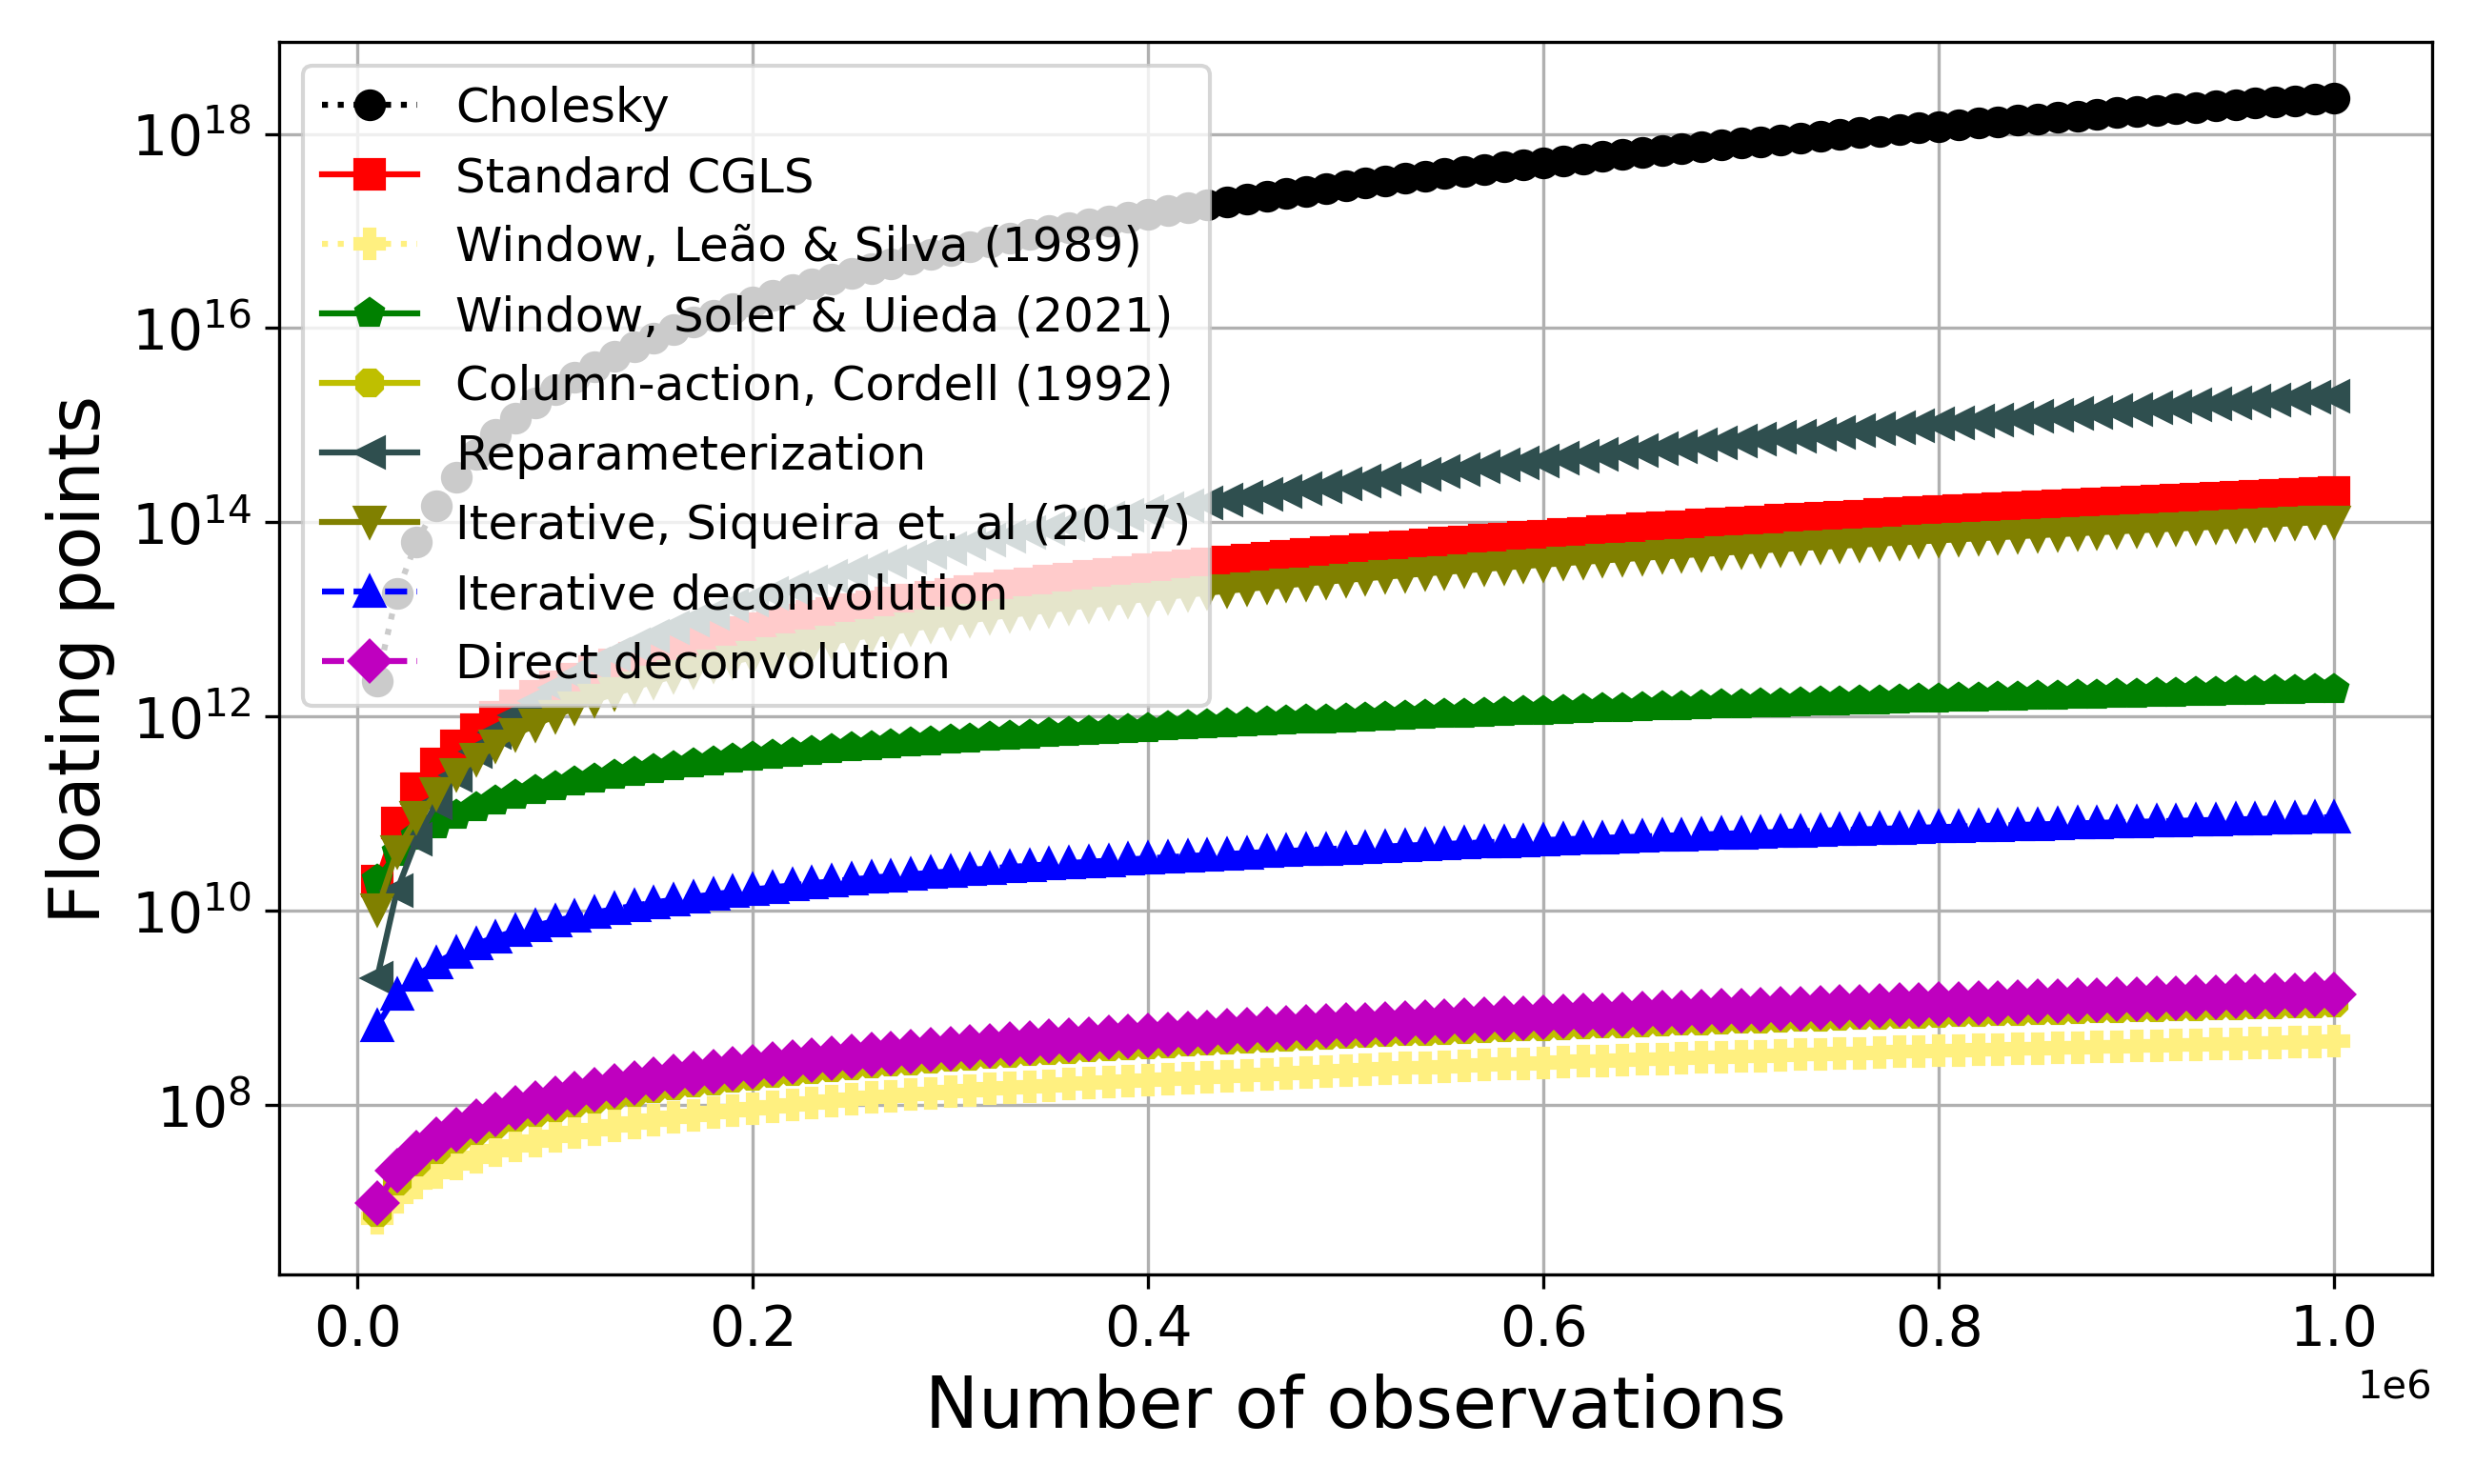
\includegraphics[width=9cm]{Fig/flops_grav}% This is a *.eps file
\end{center}
\caption{Number of \textit{flops} for many of the methods described in this work to estimate the equivalent sources using gravity data. The range of observations varies from $10,000$ to $1,000,000$.}
\label{fig:1}
\end{figure}

%\begin{figure}[htbp]
%	\begin{center}
%		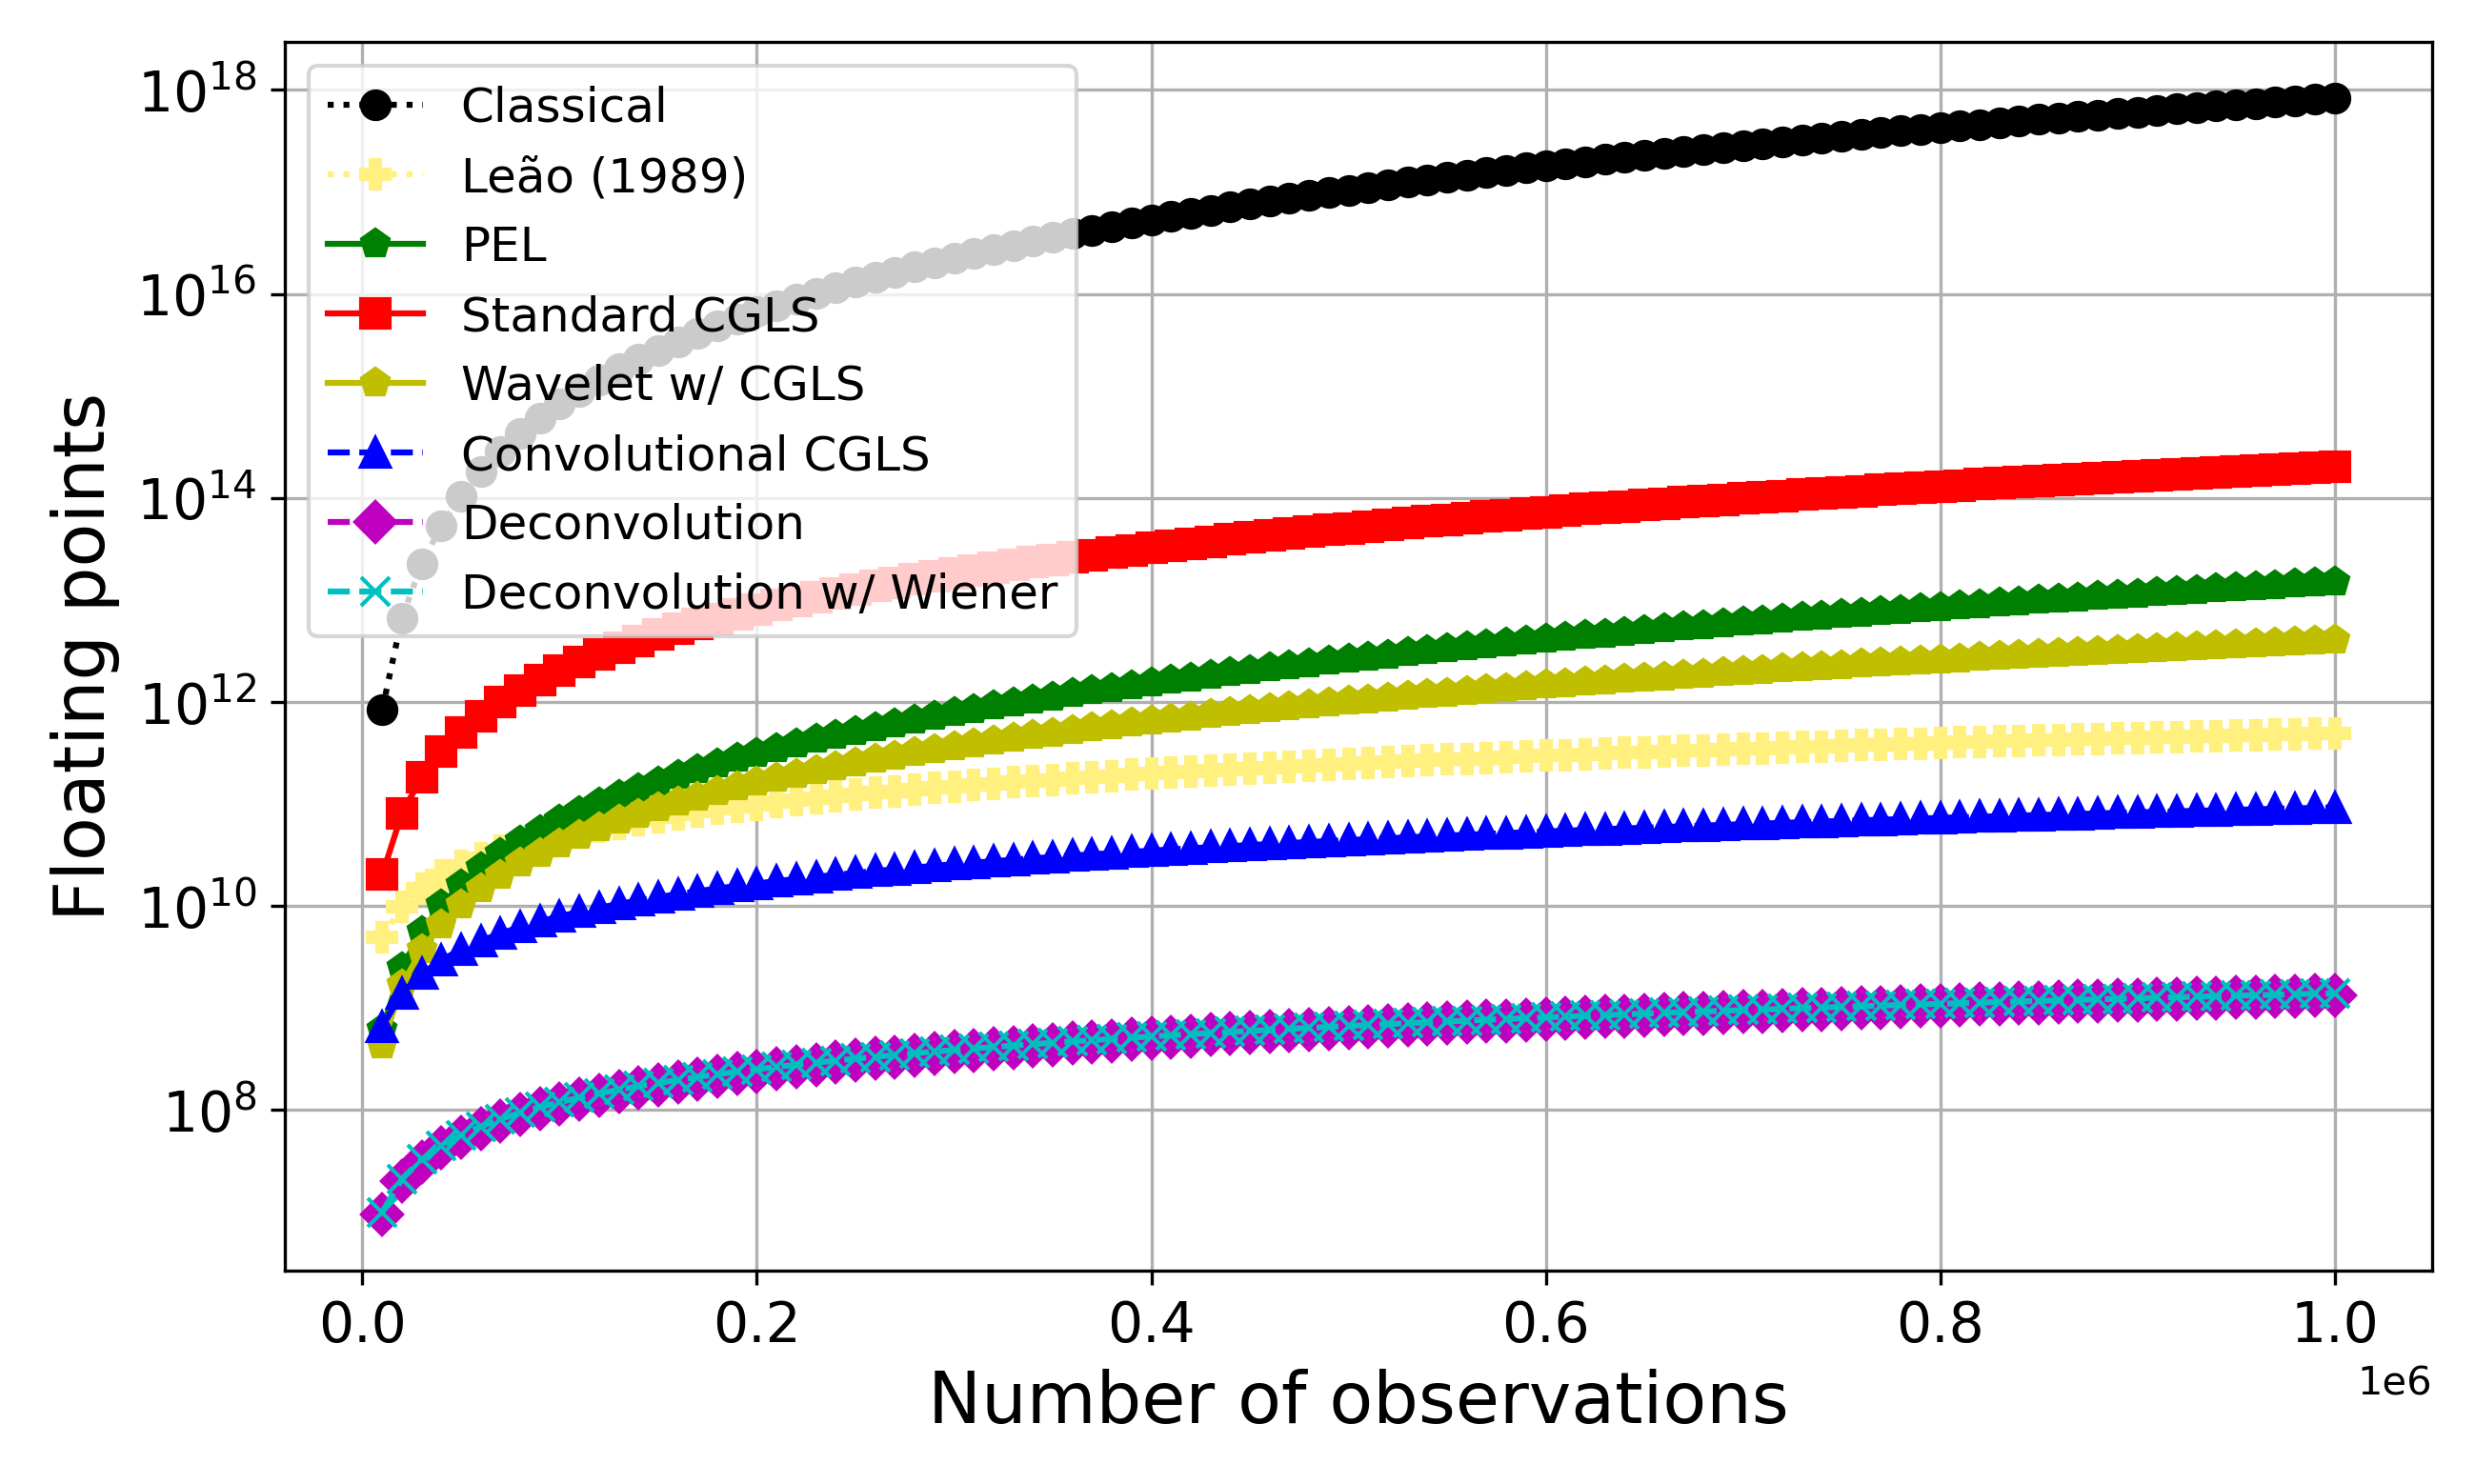
\includegraphics[width=9cm]{Fig/flops_mag}% This is a *.eps file
%	\end{center}
%	\caption{Number of \textit{flops} for many of the methods described in this work to estimate the equivalent sources using magnetic data. The range of observations varies from $10,000$ to $1,000,000$.}
%	\label{fig:2}
%\end{figure}

\begin{figure}[htbp]
	\begin{center}
		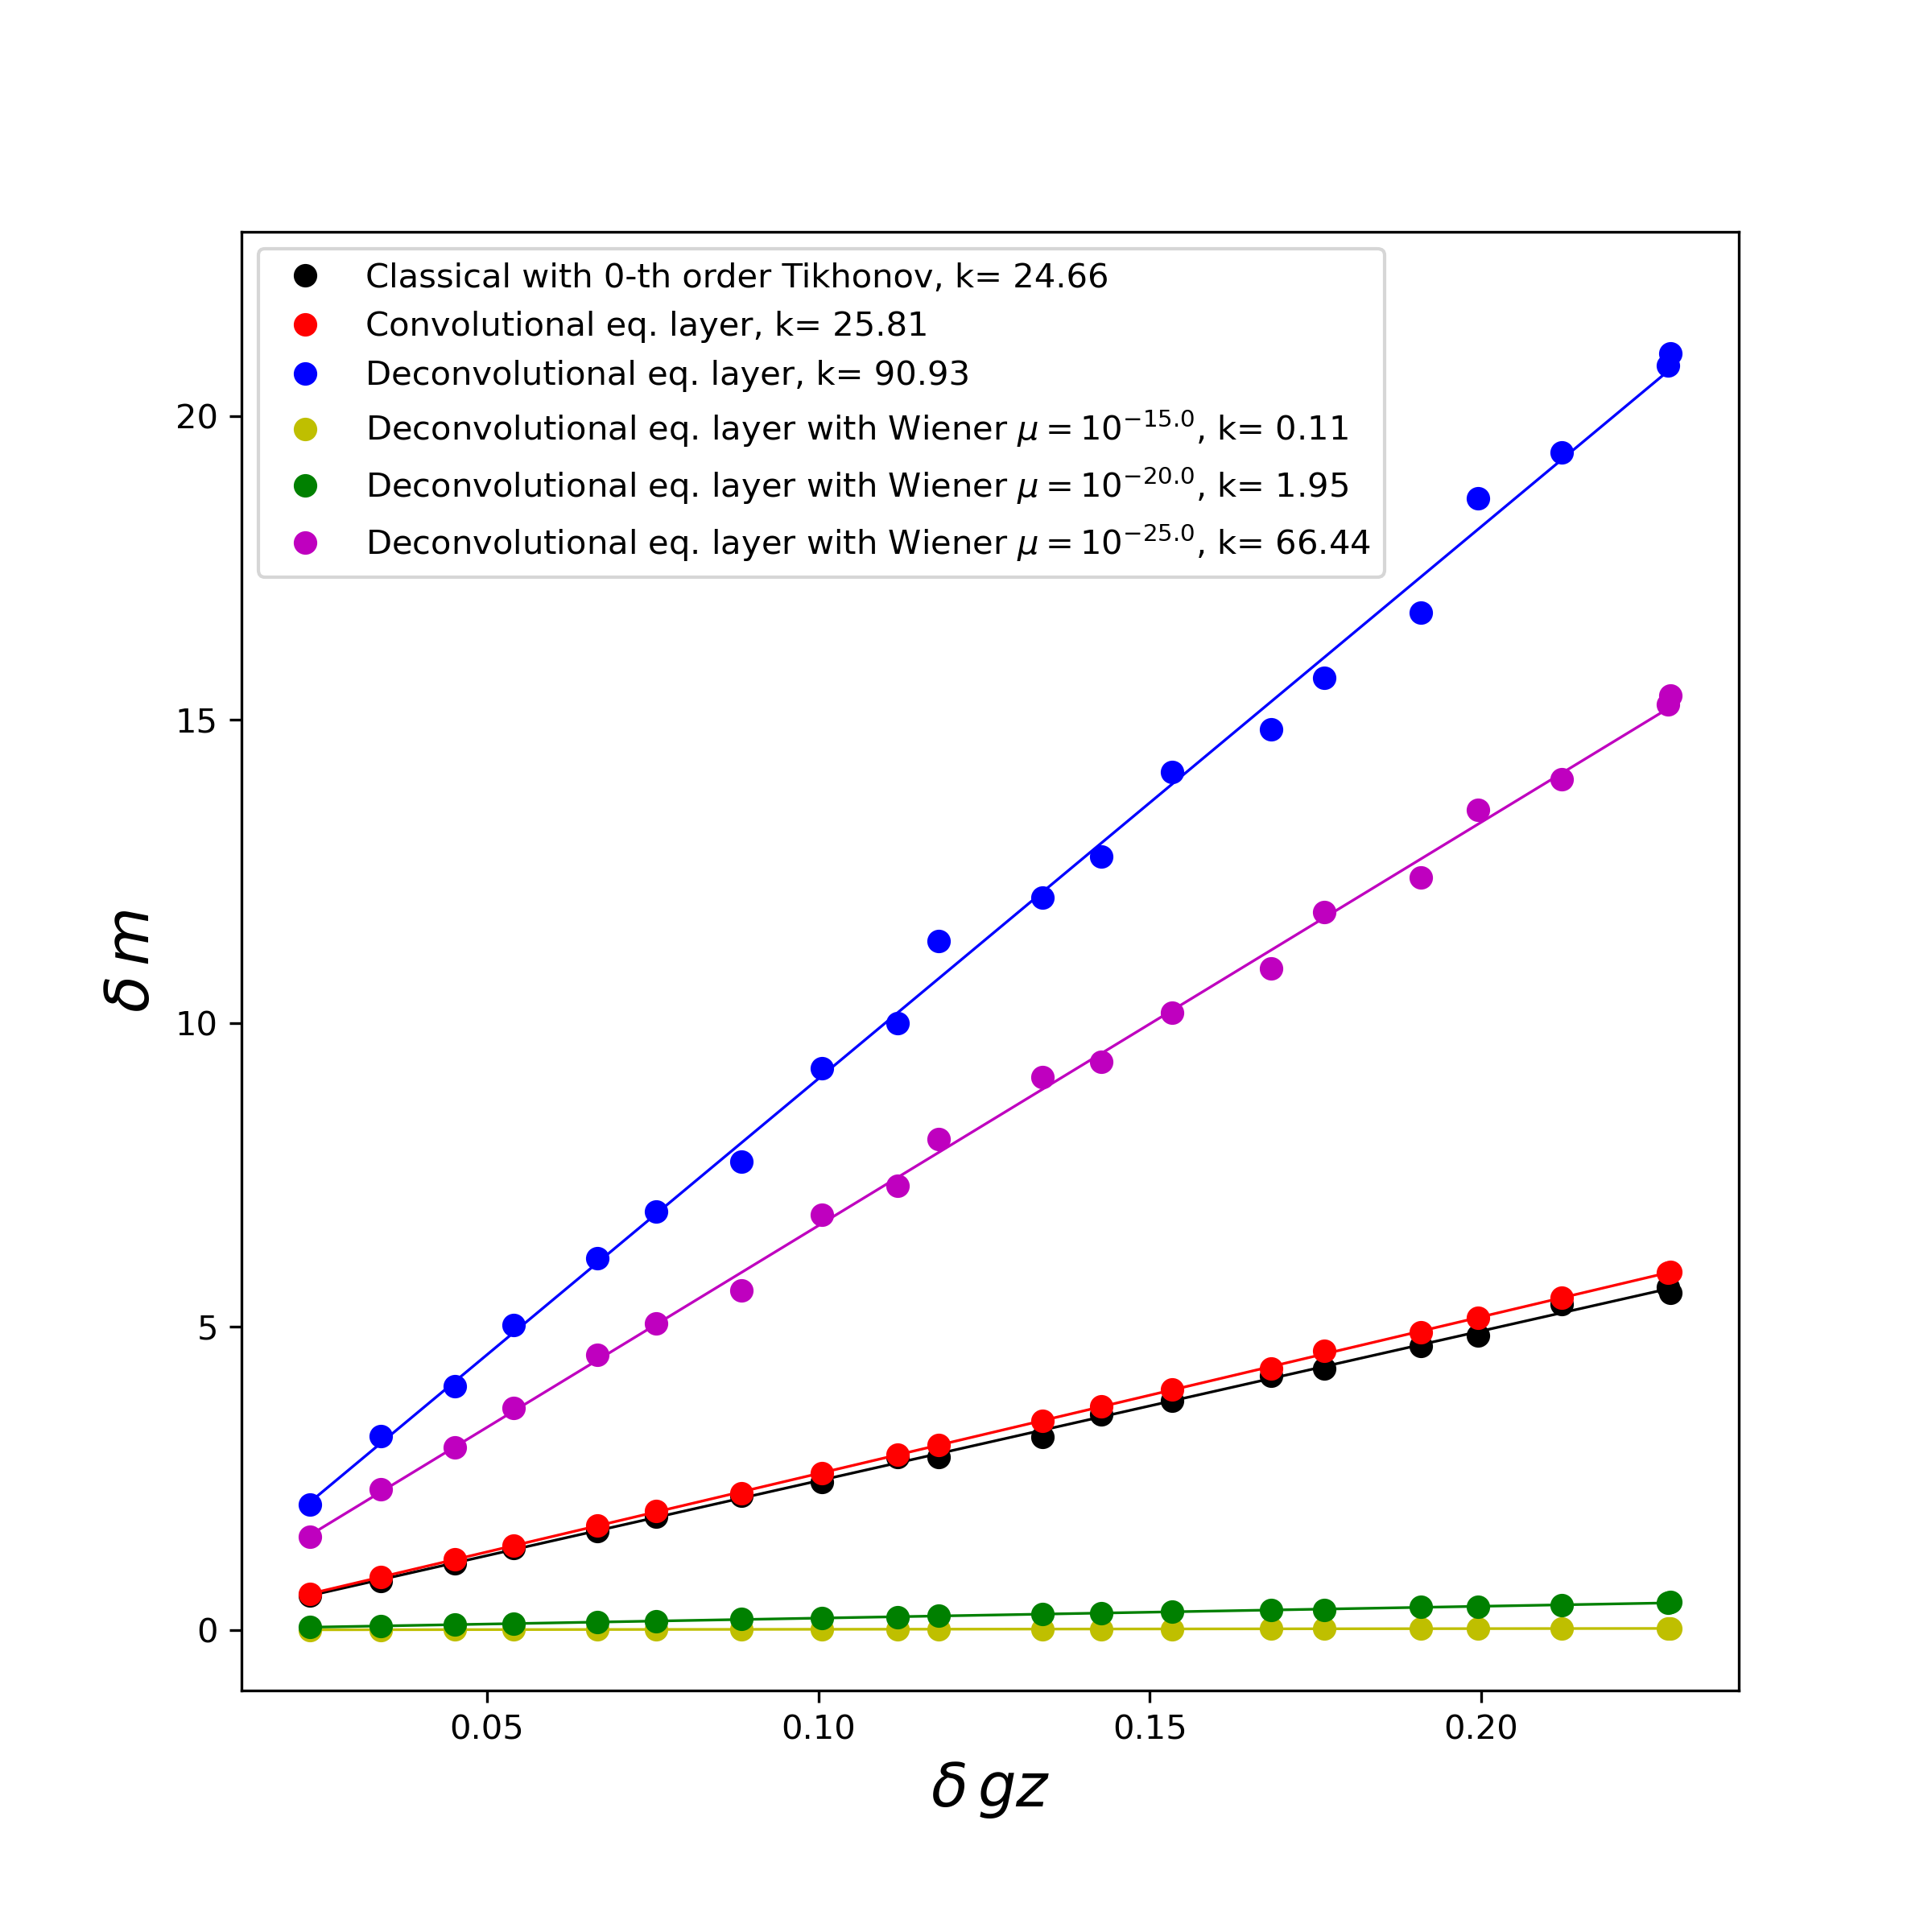
\includegraphics[width=9cm]{Fig/stability_grav}
	\end{center}
	\caption{Stability analysis of some of the equivalent layer methods of the gravimetric case.}
	\label{fig:3}
\end{figure}

\begin{figure}[htbp]
	\begin{center}
		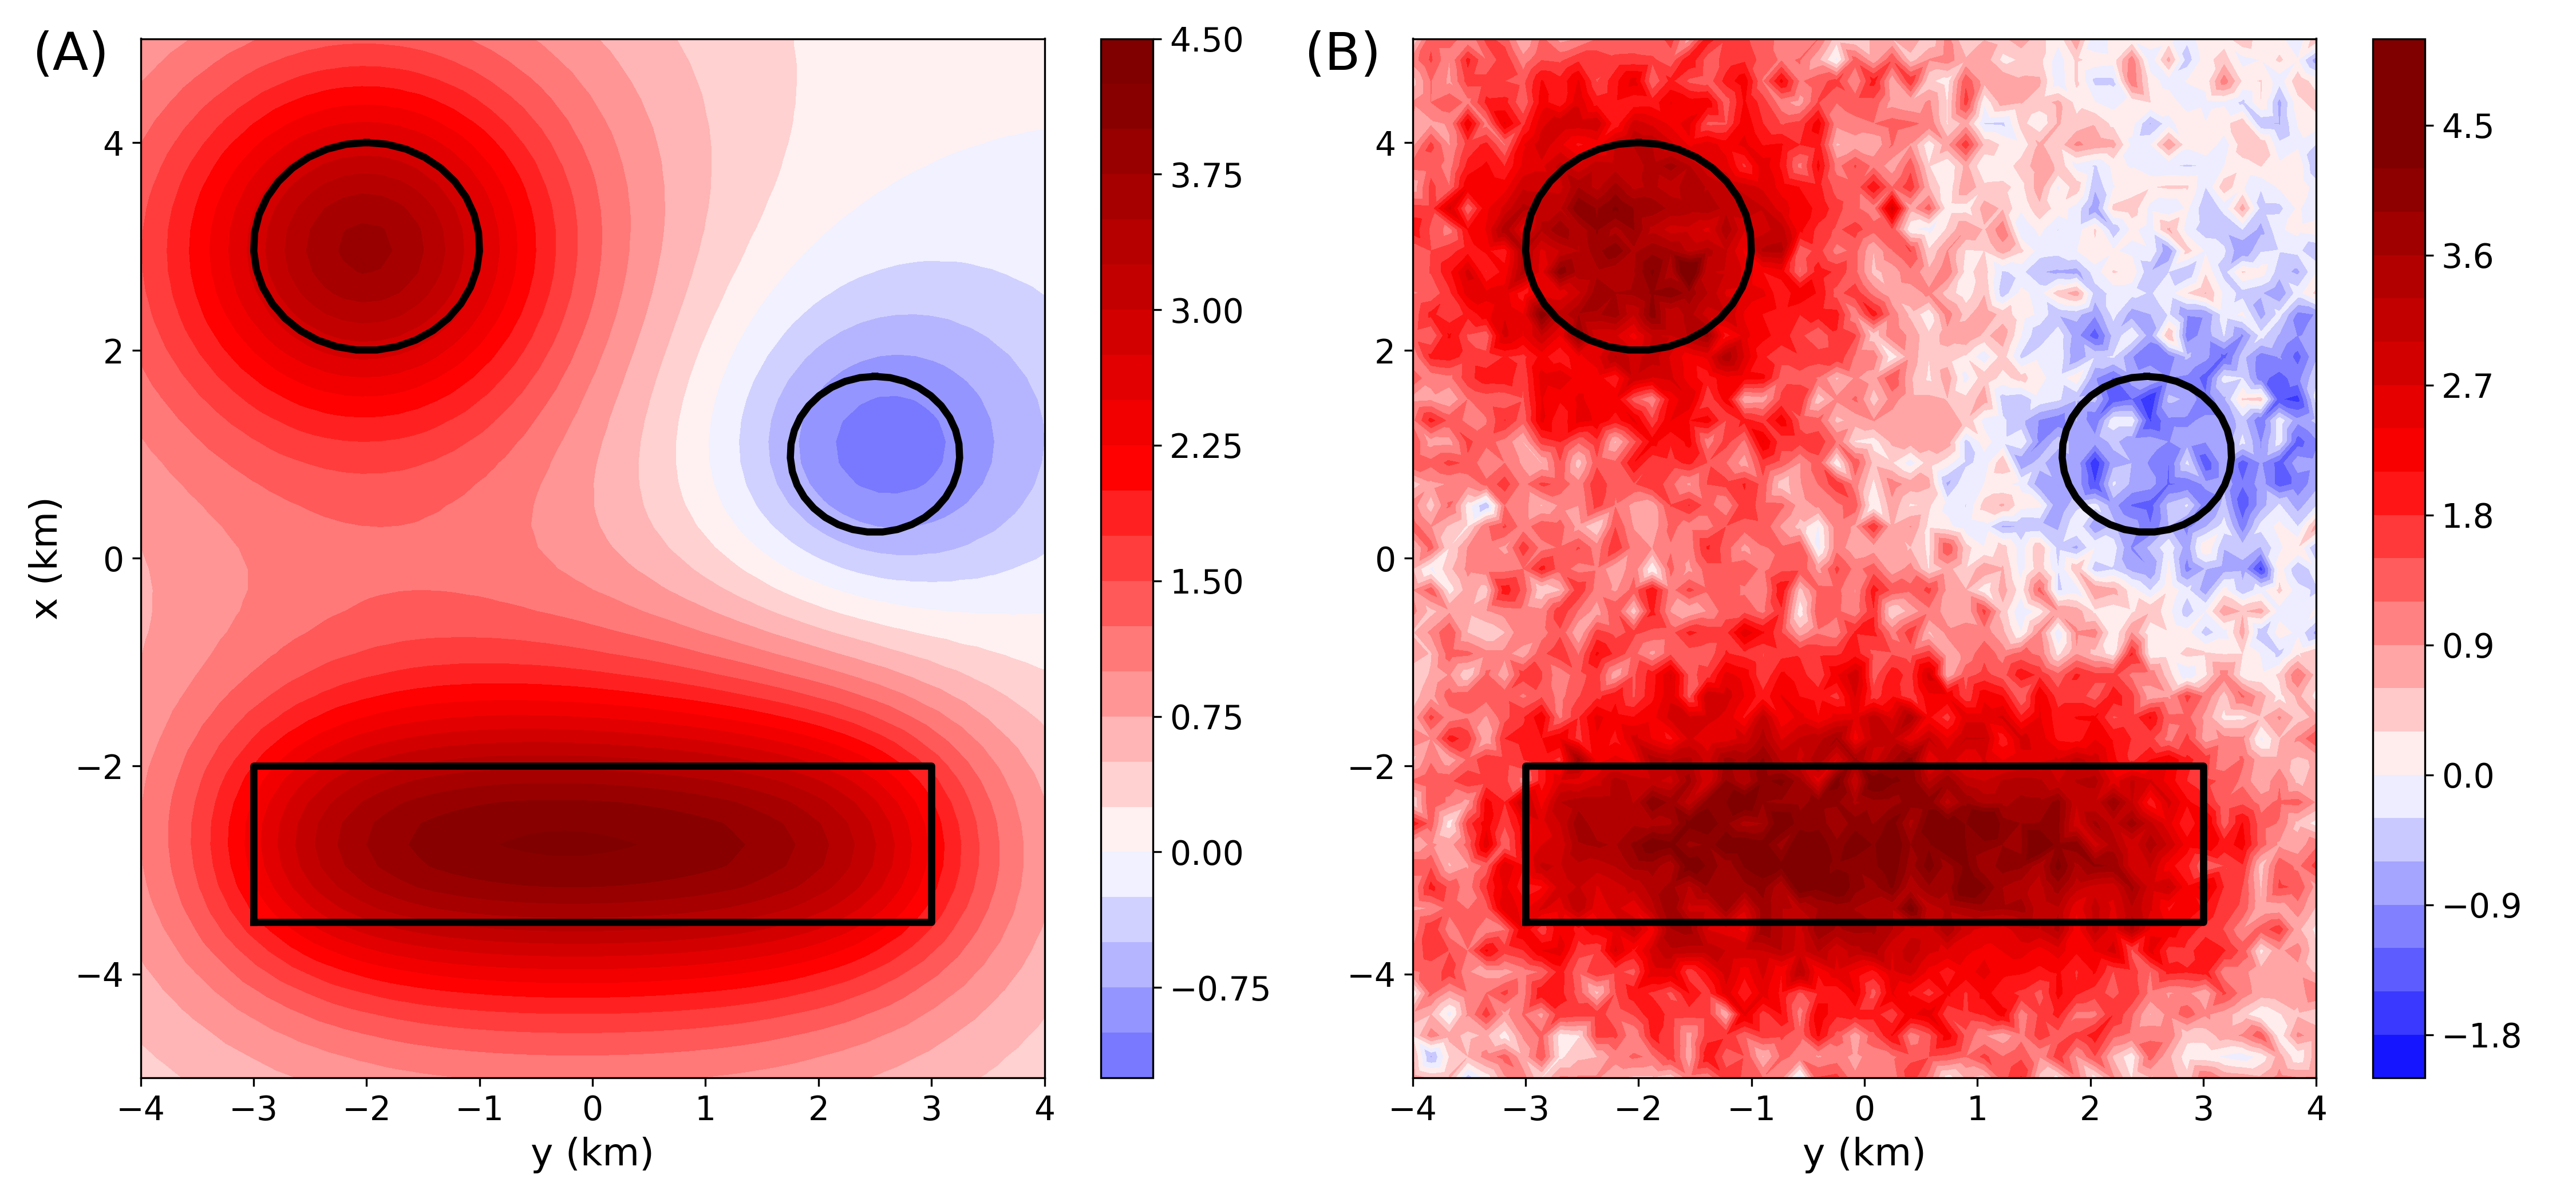
\includegraphics[width=9cm]{Fig/synthetic_grav}
	\end{center}
	\caption{Synthetic data of the gravimetric case. The observations points are placed in a regular grid of $50 \times 50$. Panel (A) shows the noise-free data and panel (B) shows the maximum noised data ($10\%$).}
	\label{fig:4}
\end{figure}

\begin{figure}[htbp]
	\begin{center}
		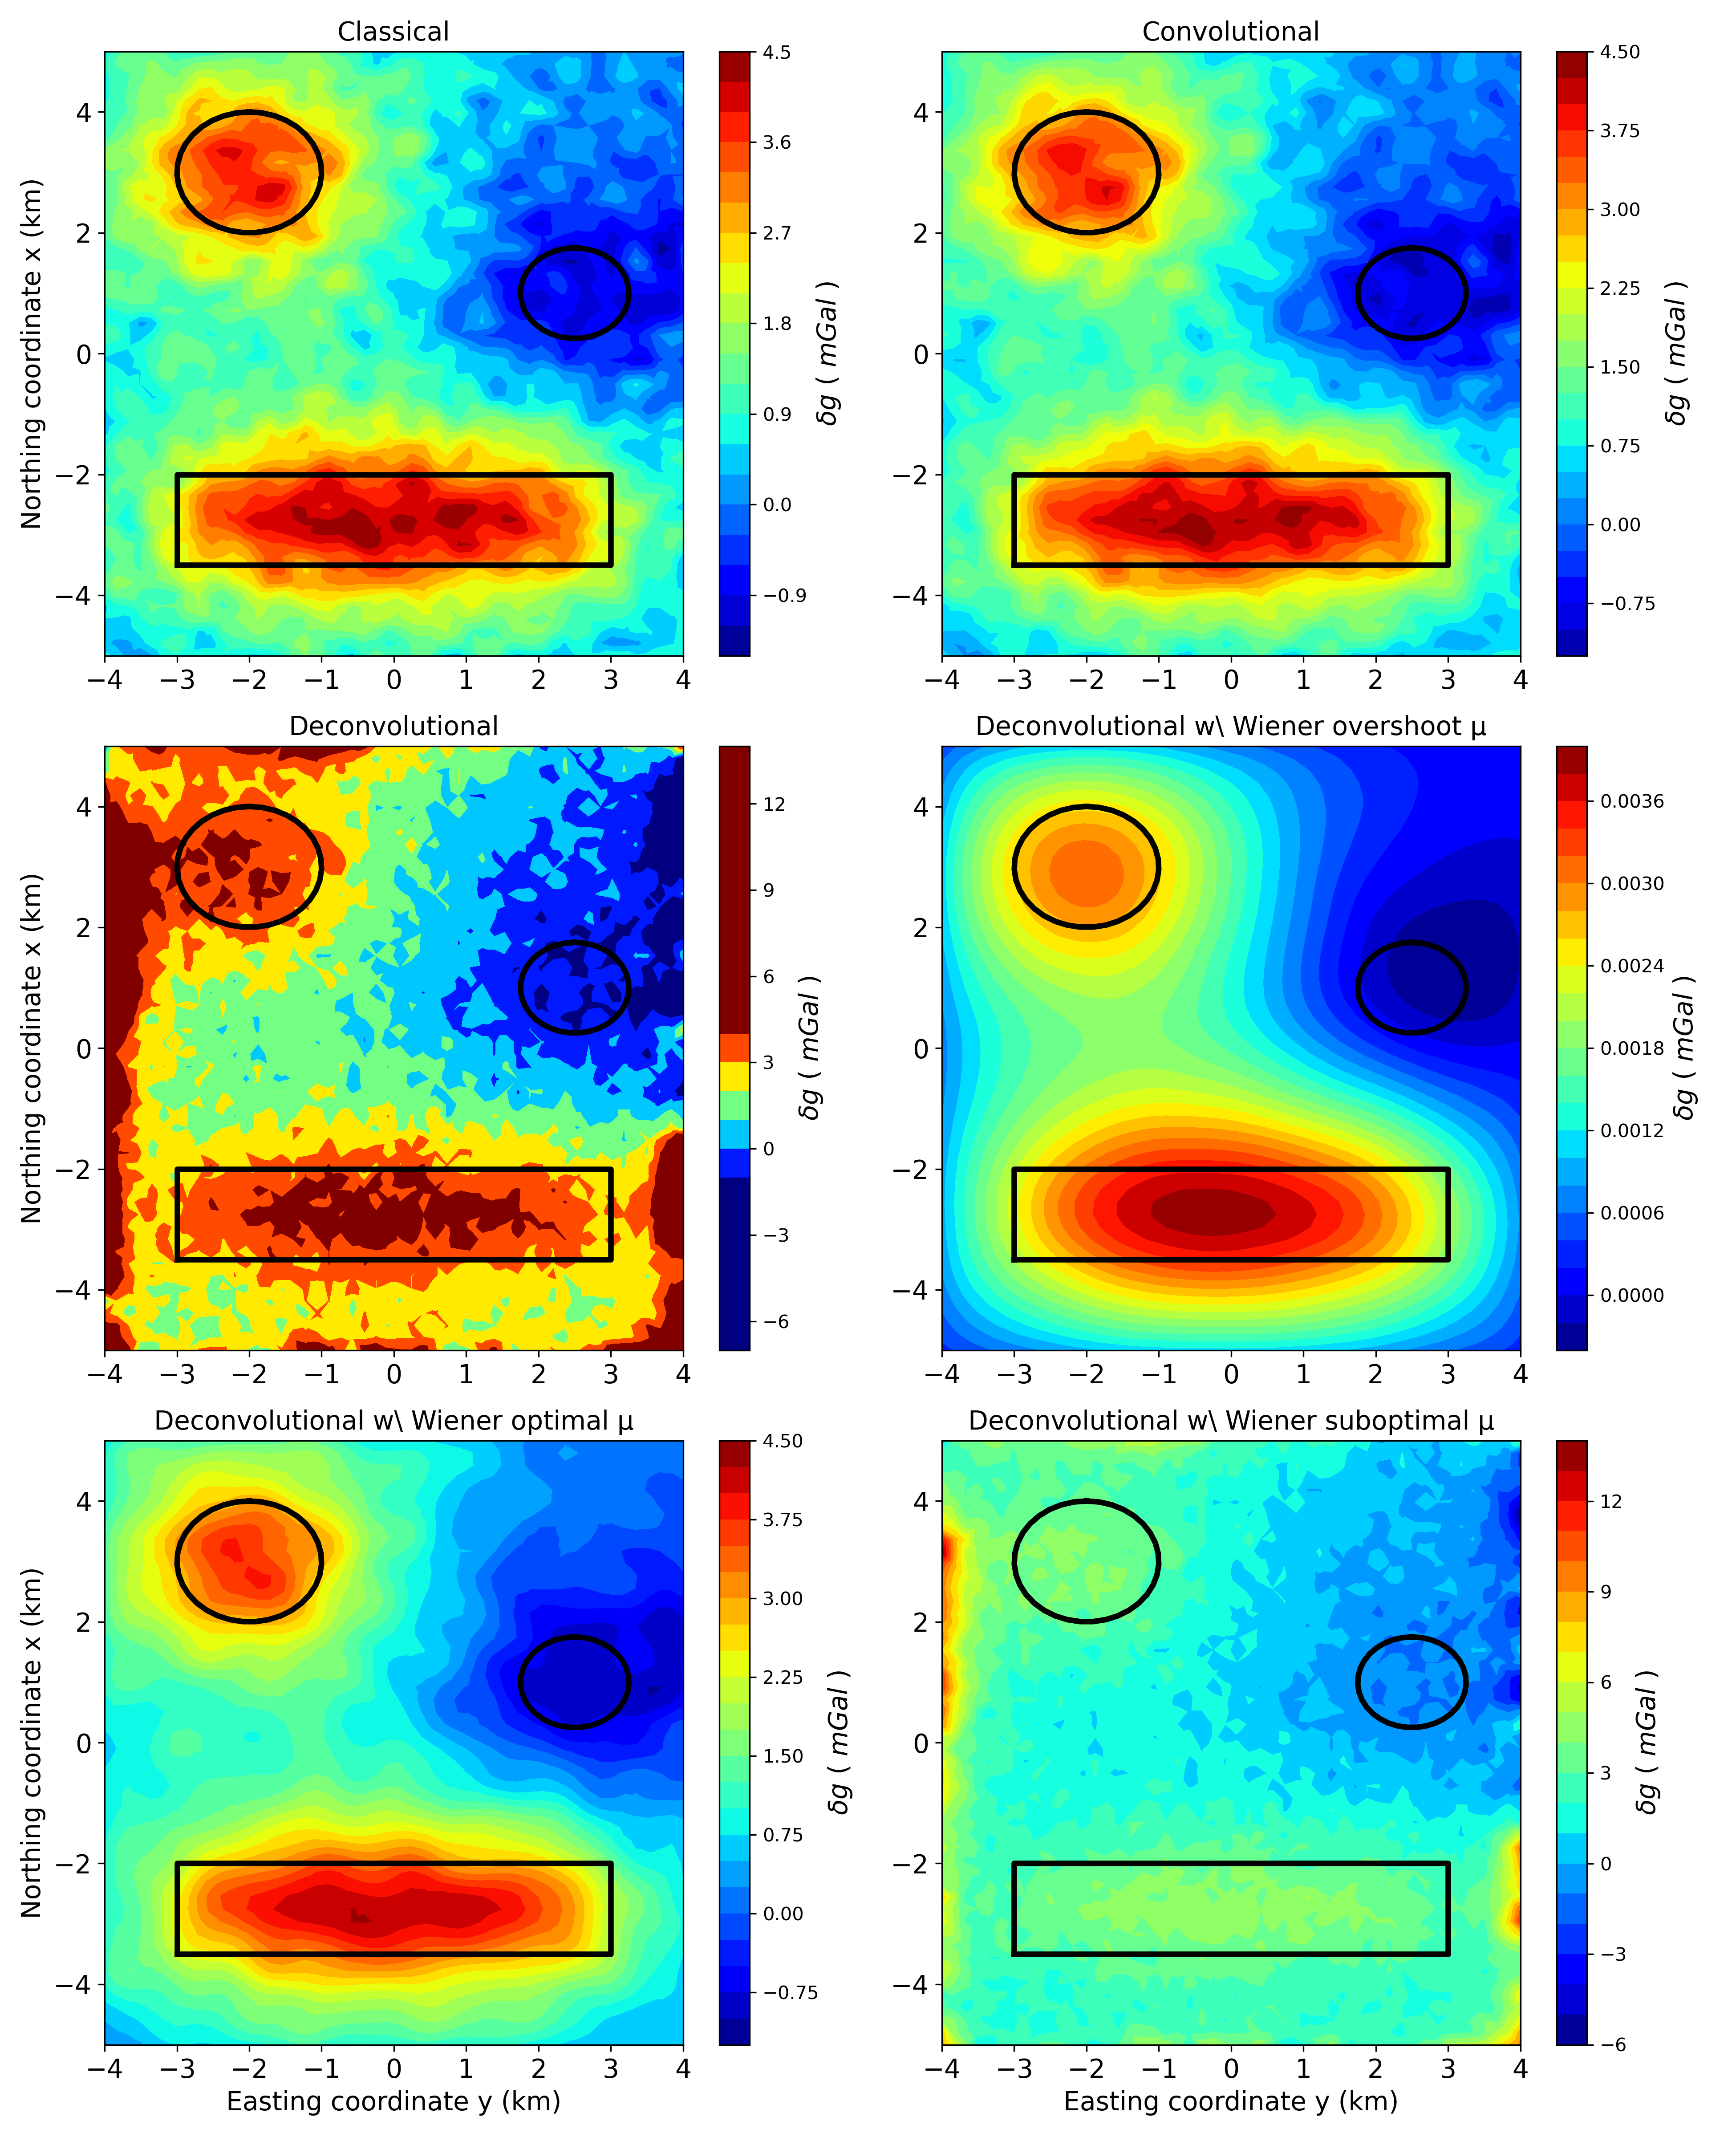
\includegraphics[width=10cm]{Fig/stability_grav_comparison}
	\end{center}
	\caption{Predicted gravity data for different methods of the equivalent layer with maximum level of noise. Panel \textbf{(A)} is the classical method, \textbf{(B)} is the convolutional, \textbf{(C)} is the deconvolutional, \textbf{(D)} is the deconvolutional method using Wiener stabilization with a too high value for $\mu$, \textbf{(E)} is the deconvolutional method using Wiener stabilization with a optimal value for $\mu$ and \textbf{(F)} is the deconvolutional method using Wiener stabilization with a too low value for $\mu$.}
	\label{fig:5}
\end{figure}

\begin{figure}[htbp]
	\begin{center}
		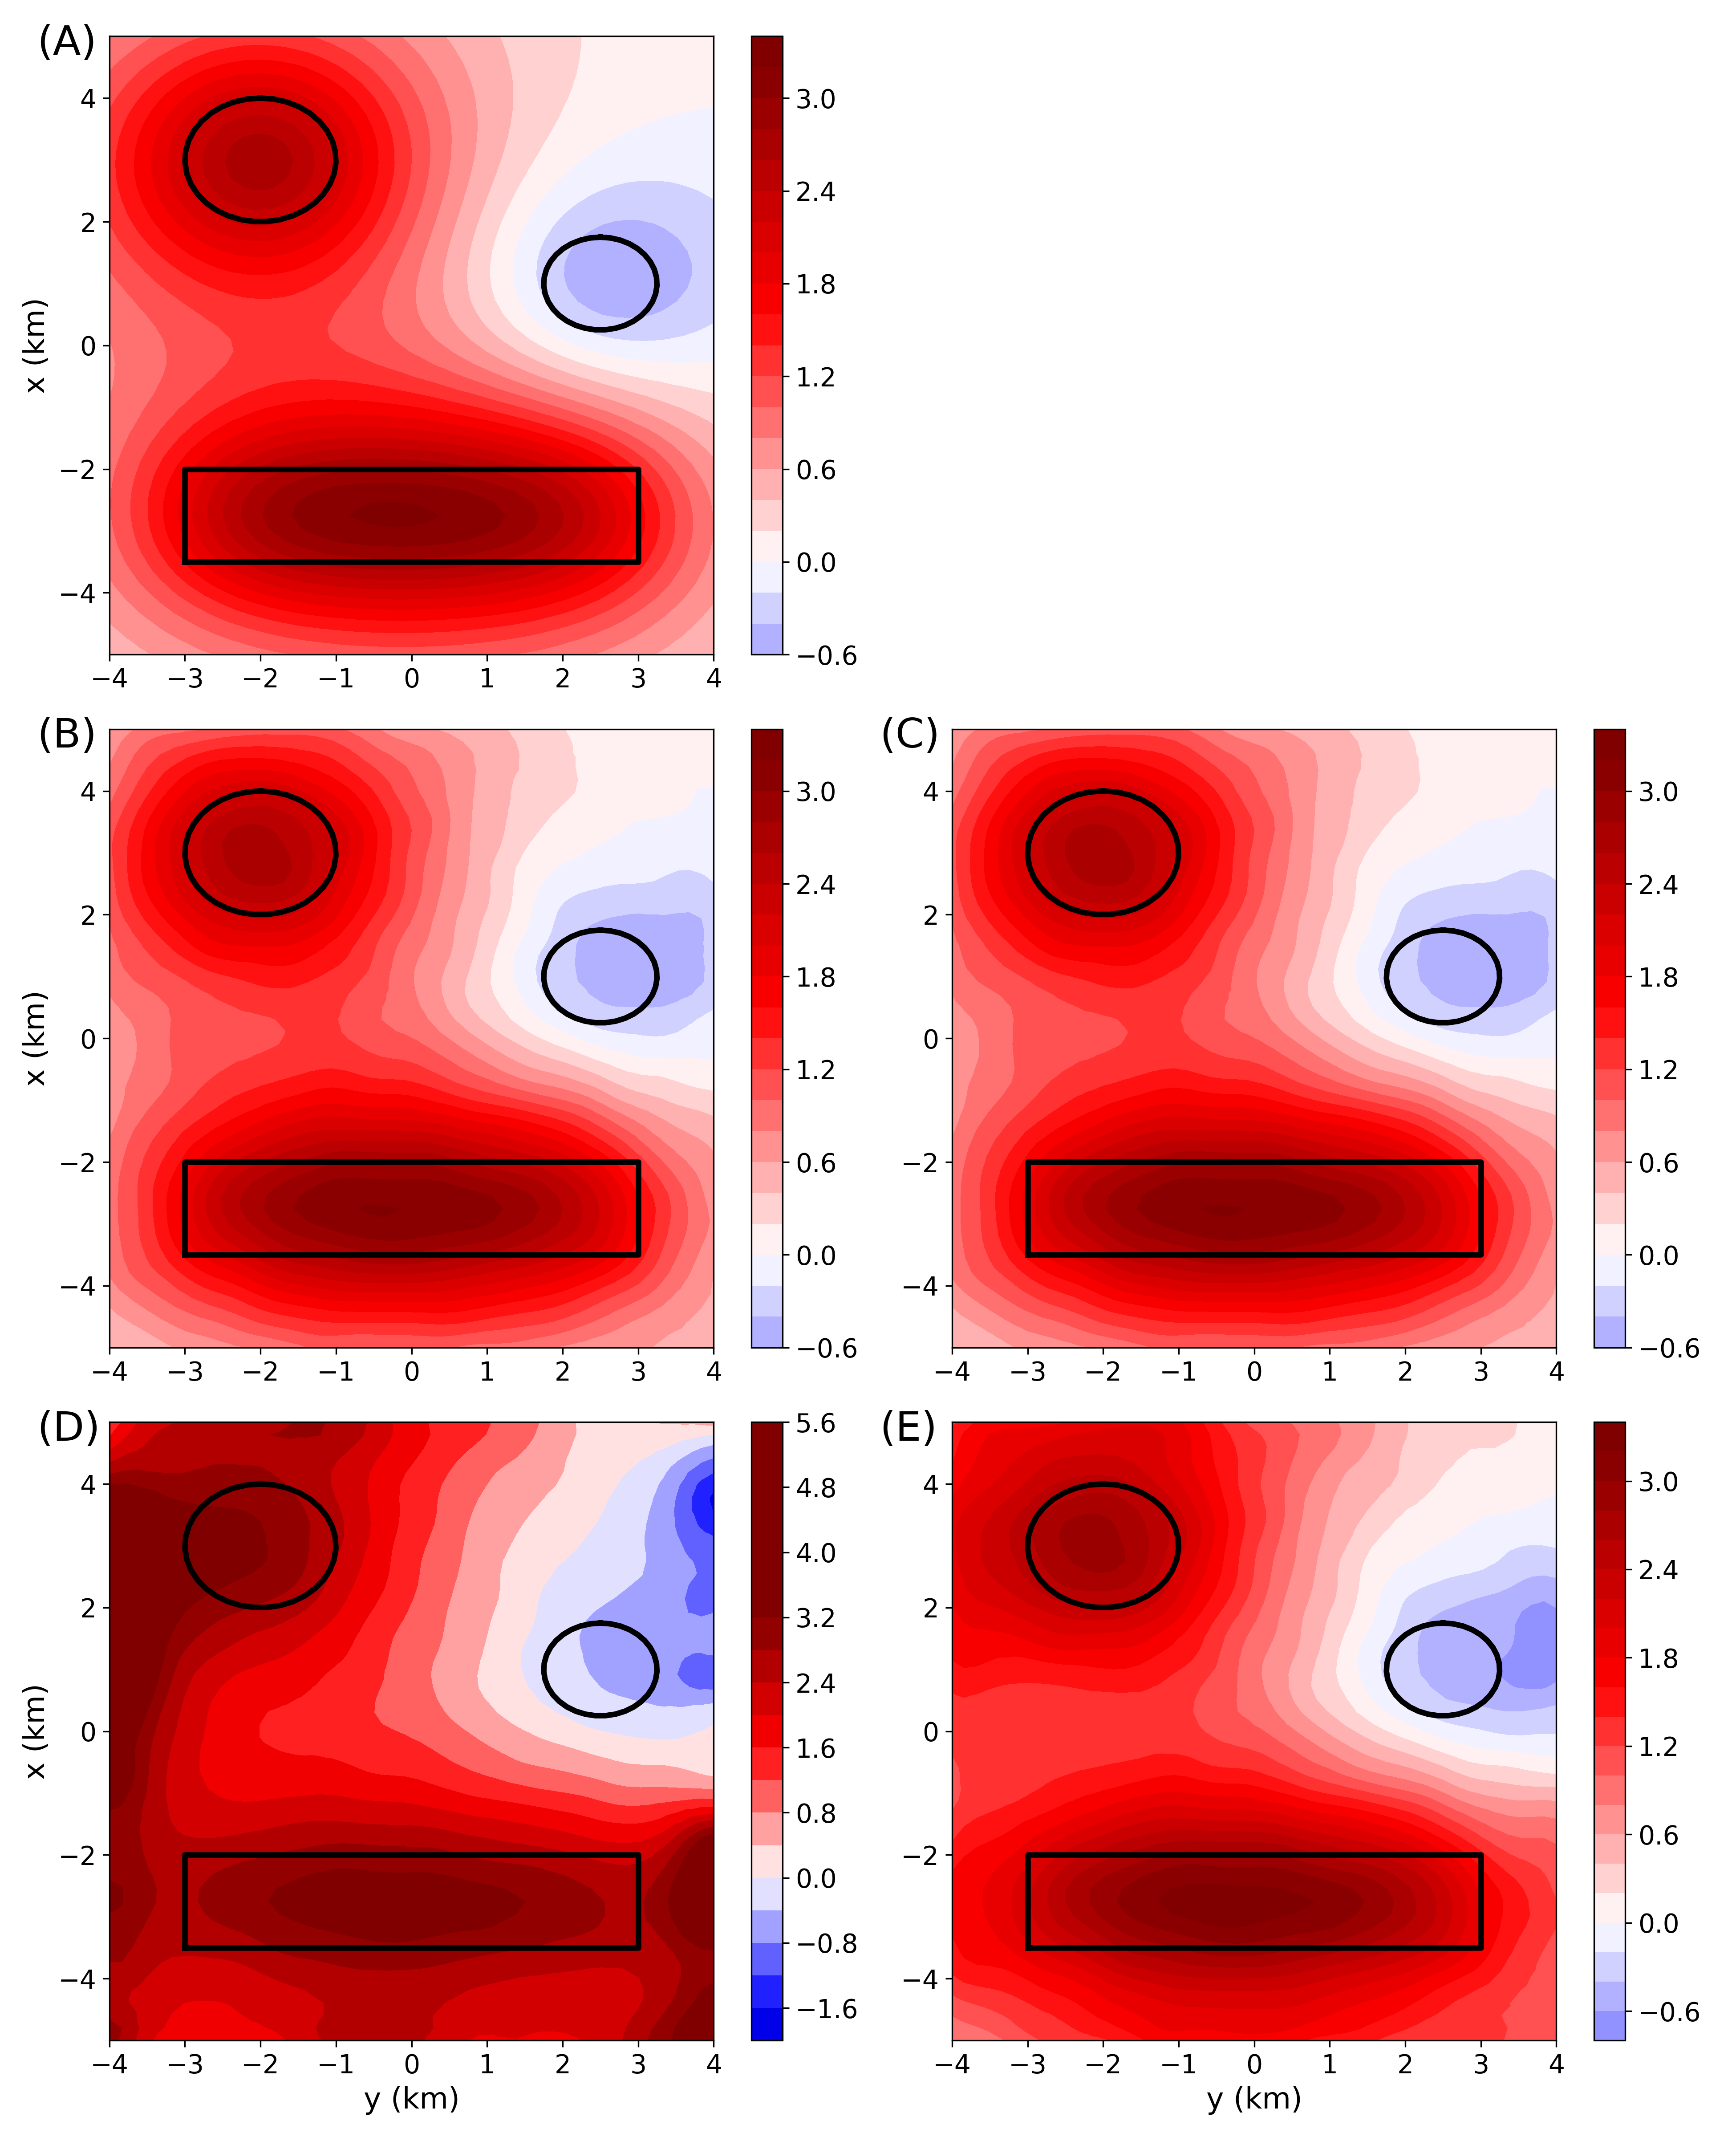
\includegraphics[width=10cm]{Fig/grav_upward}
	\end{center}
	\caption{True noiseless upward gravimetric data at $z_i = -500$ m height and predicted data for different methods of the equivalent layer with maximum level of noise. Panel \textbf{(A)} is the true upward gravity data, Panel \textbf{(B)} is the classical method, \textbf{(C)} is the convolutional, \textbf{(D)} is the deconvolutional, \textbf{(E)} is the deconvolutional method using Wiener stabilization with a optimal value for $\mu = 10^{-20}$.}
	\label{fig:grav_up}
\end{figure}

\begin{figure}[htbp]
	\begin{center}
		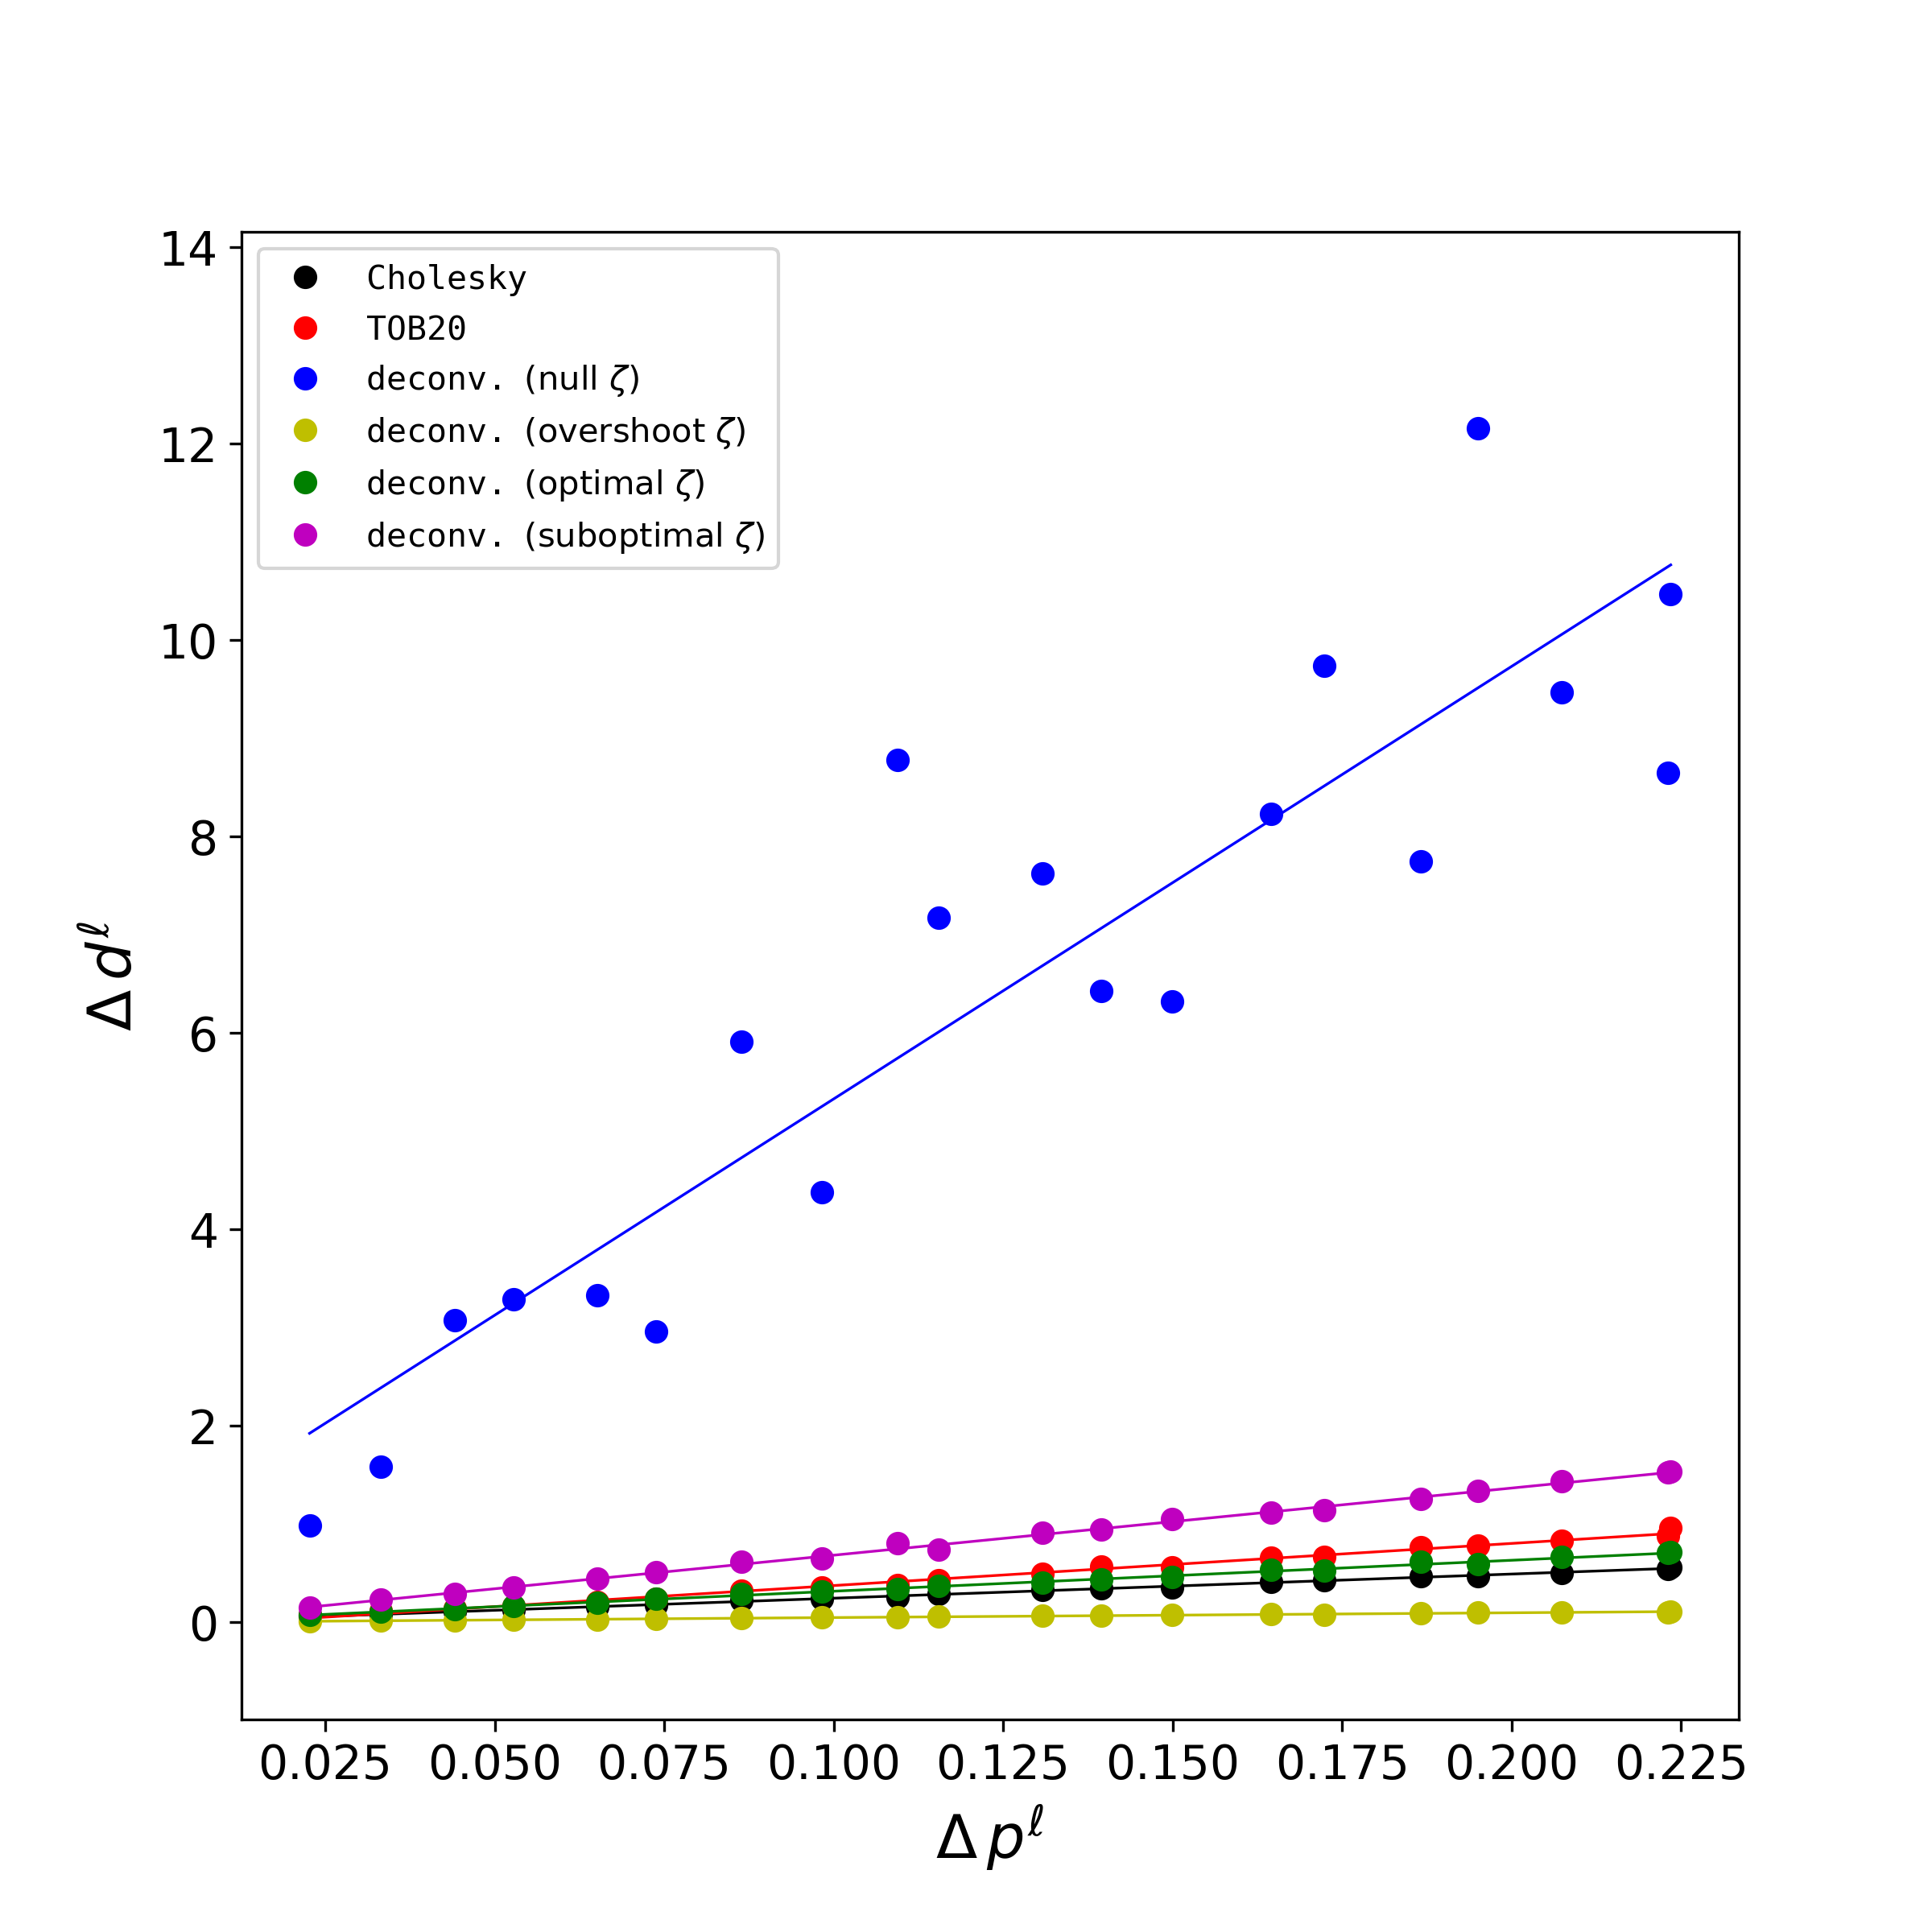
\includegraphics[width=10cm]{Fig/stability_mag}
	\end{center}
	\caption{Stability analysis of some of the equivalent layer methods of the magnetic case.}
	\label{fig:6}
\end{figure}

\begin{figure}[htbp]
	\begin{center}
		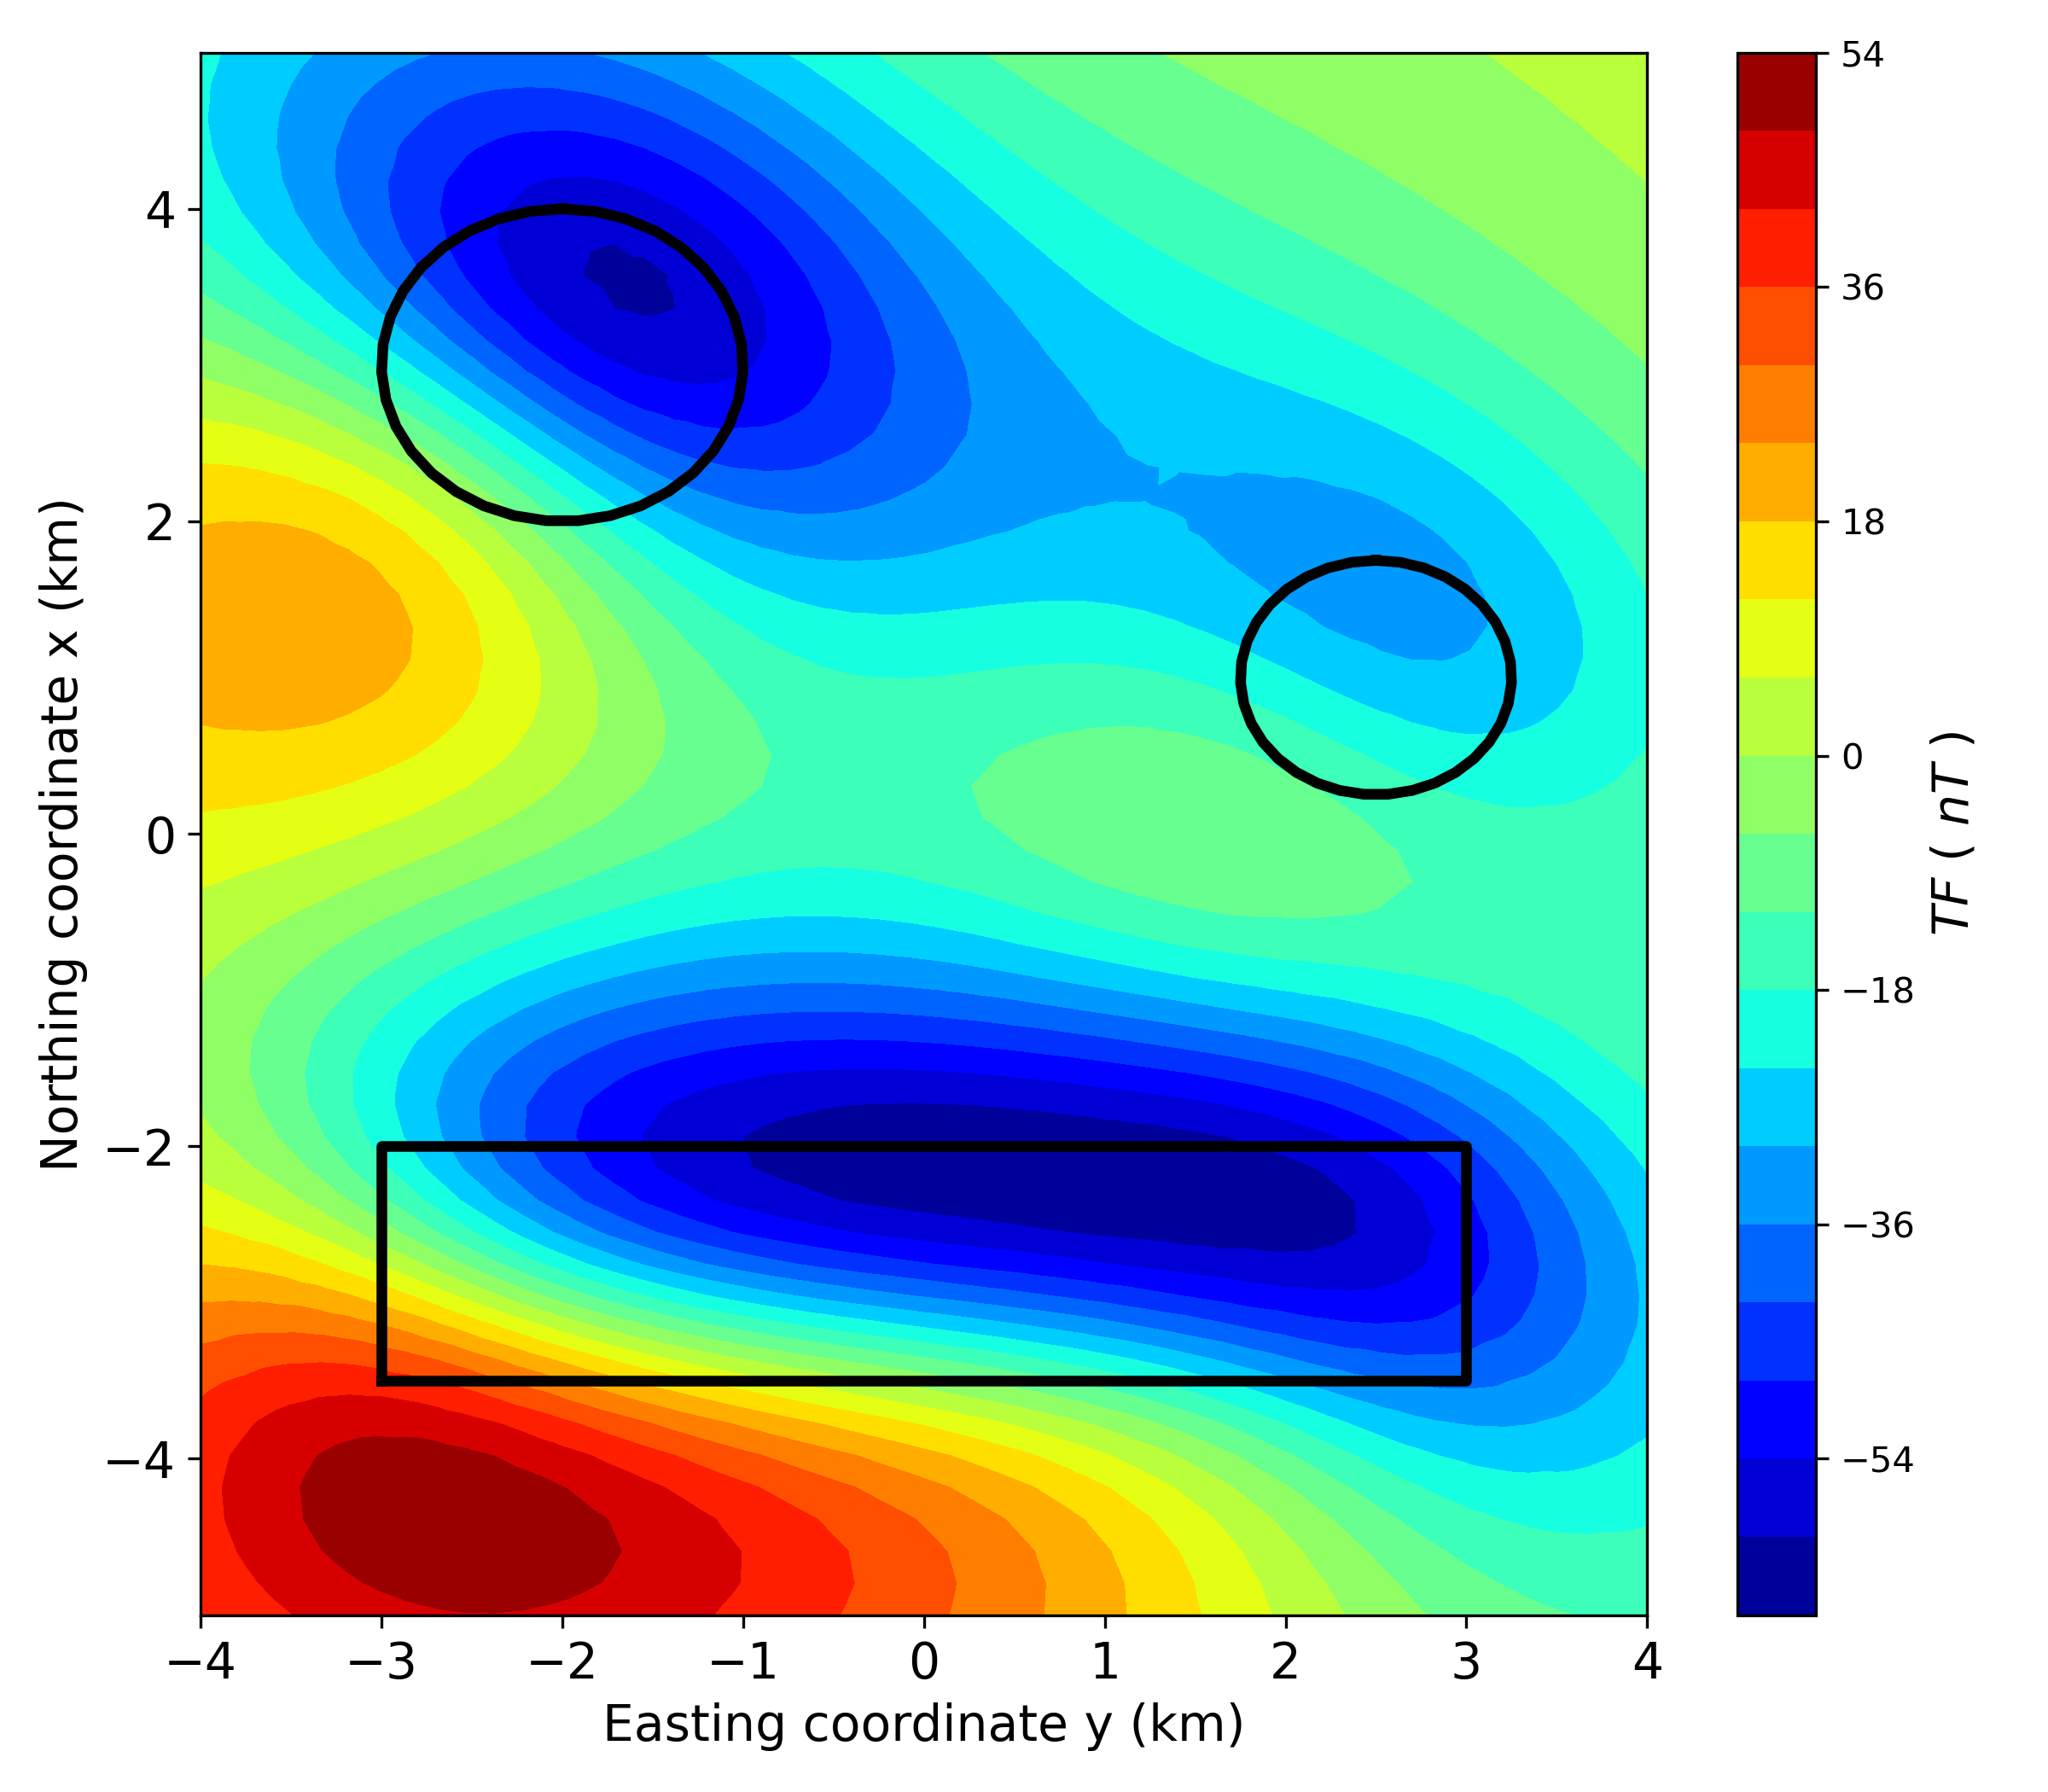
\includegraphics[width=10cm]{Fig/synthetic_mag}
	\end{center}
	\caption{Synthetic data of the magnetic case. The observations points are placed in a regular grid of $50 \times 50$. Panel (A) shows the noise-free data and panel (B) shows the maximum noised data ($10\%$).}
	\label{fig:7}
\end{figure}

\begin{figure}[htbp]
	\begin{center}
		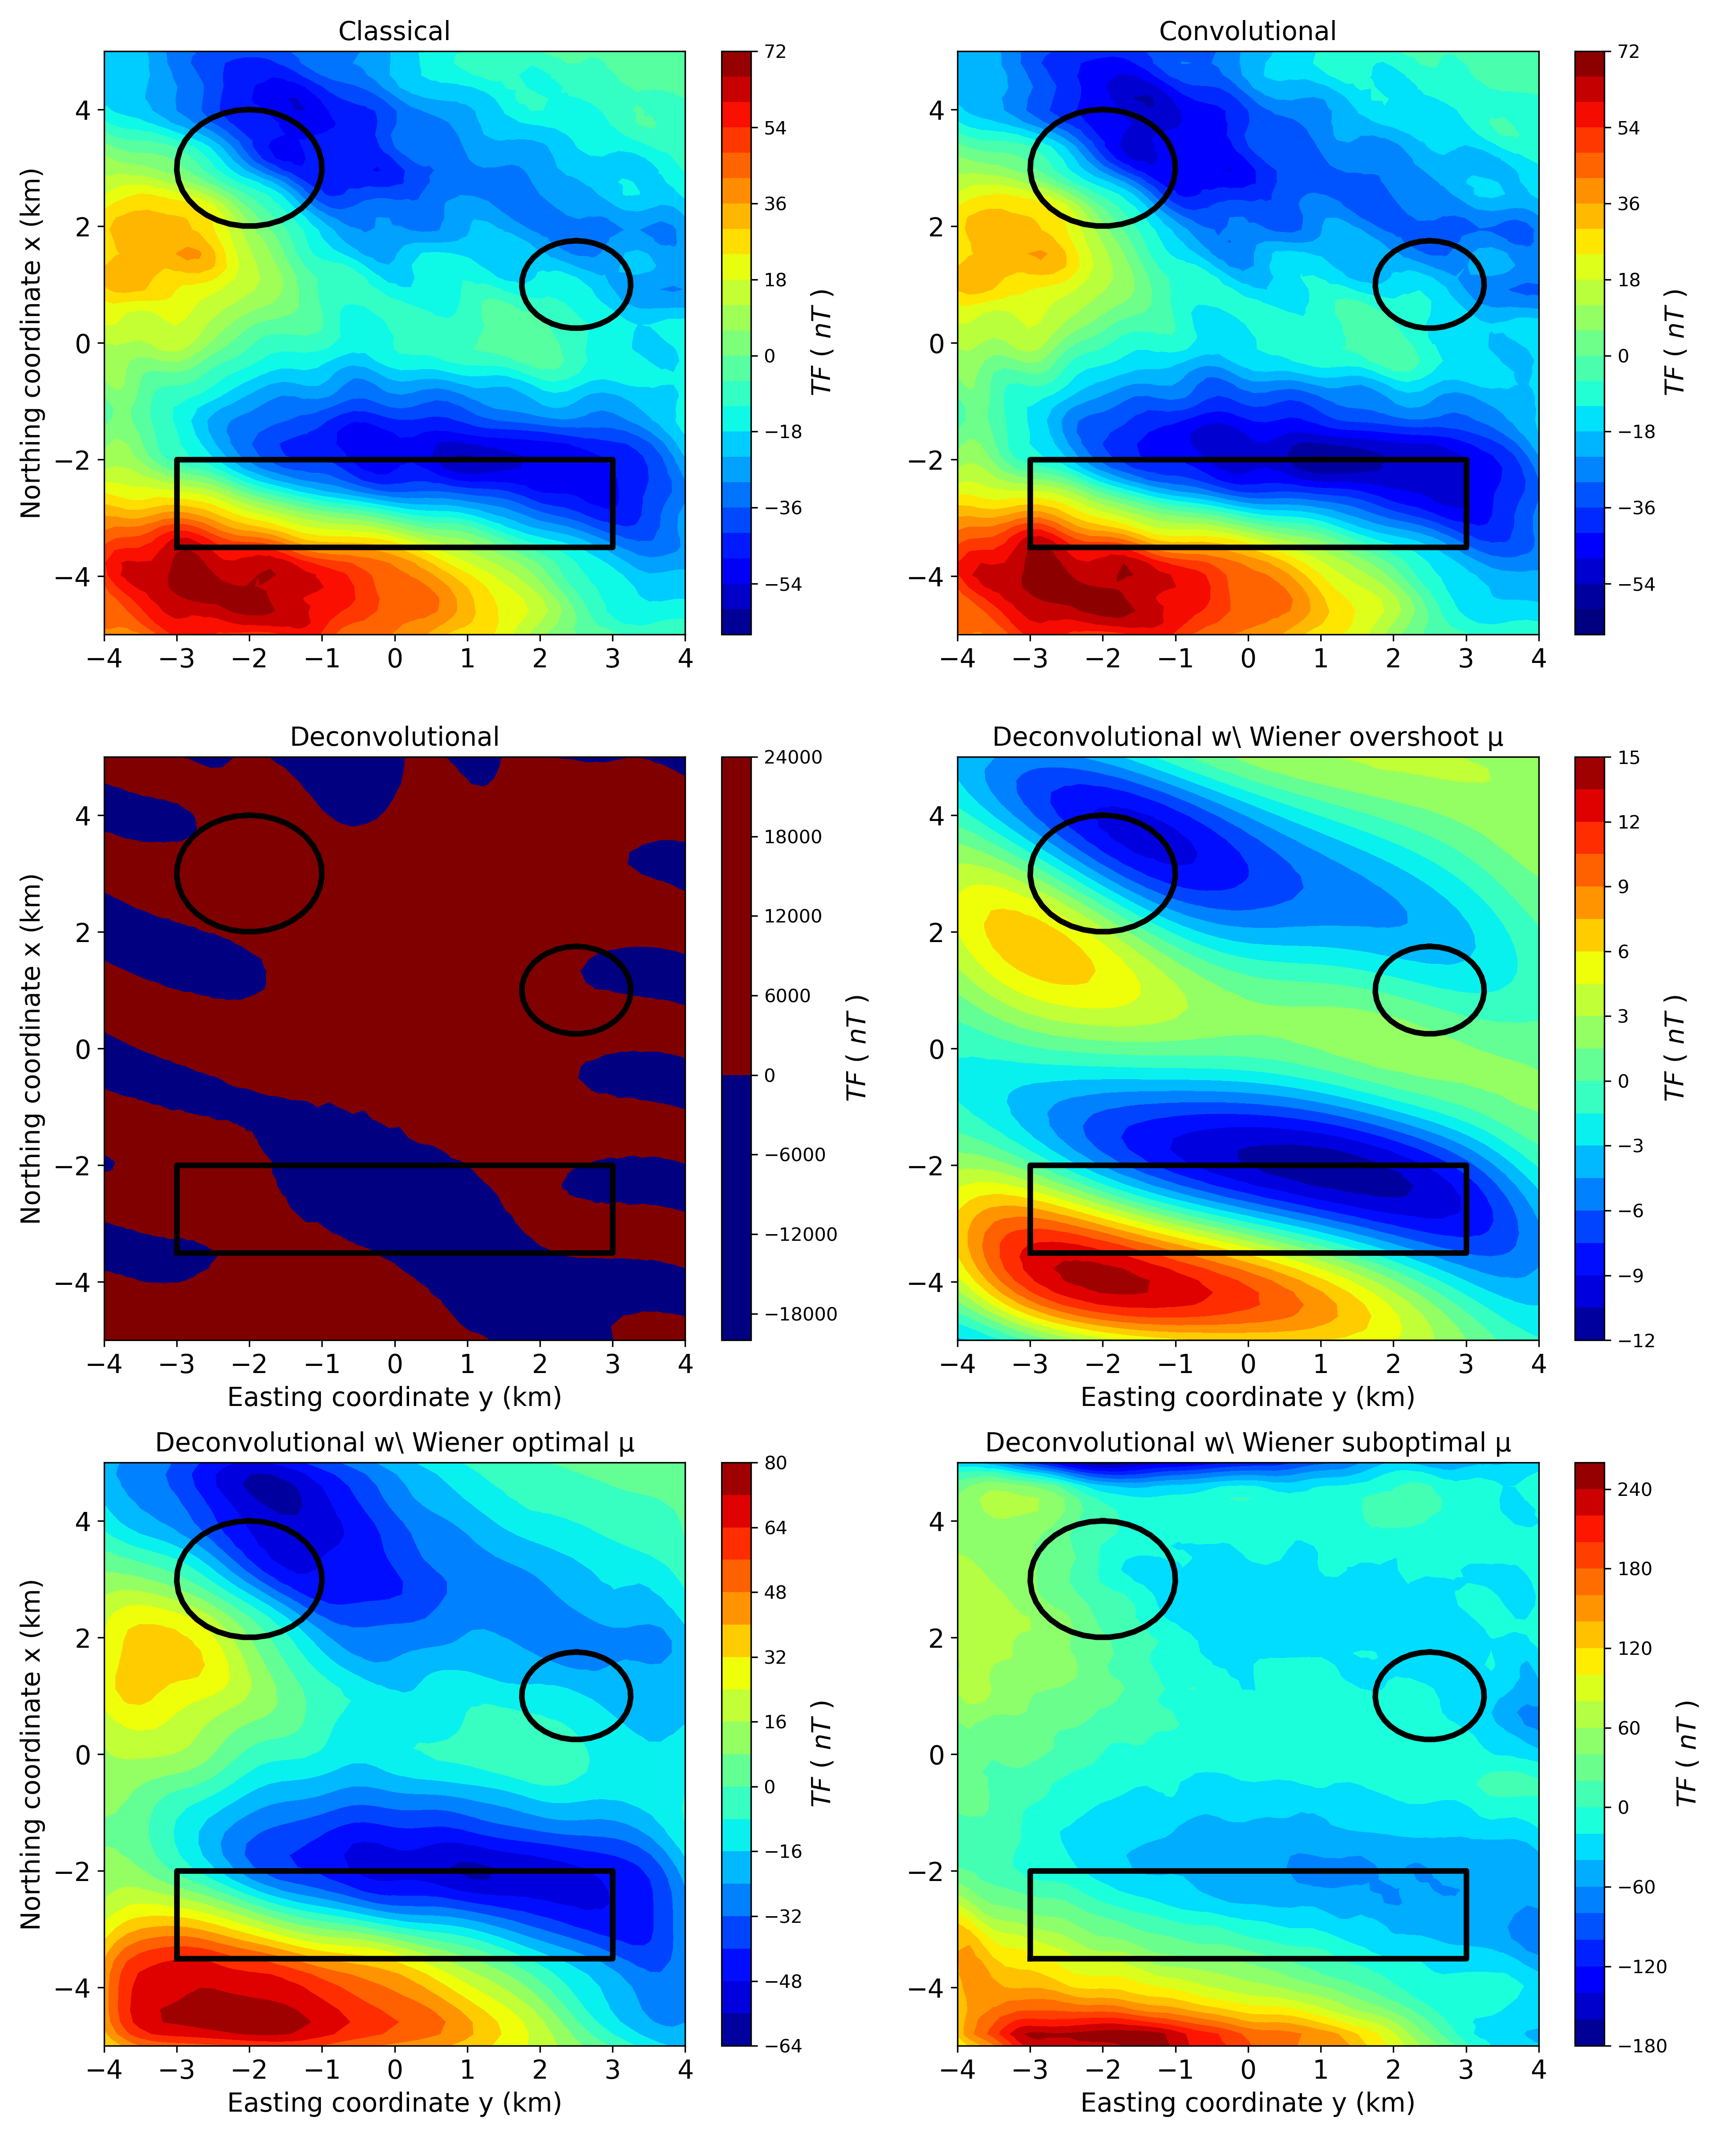
\includegraphics[width=10cm]{Fig/stability_mag_comparison}
	\end{center}
	\caption{Predicted magnetic data for different methods of the equivalent layer with maximum level of noise. Panel \textbf{(A)} is the classical method, \textbf{(B)} is the convolutional, \textbf{(C)} is the deconvolutional, \textbf{(D)} is the deconvolutional method using Wiener stabilization with a too high value for $\mu$, \textbf{(E)} is the deconvolutional method using Wiener stabilization with a optimal value for $\mu$ and \textbf{(F)} is the deconvolutional method using Wiener stabilization with a too low value for $\mu$.}
	\label{fig:8}
\end{figure}

\begin{figure}[htbp]
	\begin{center}
		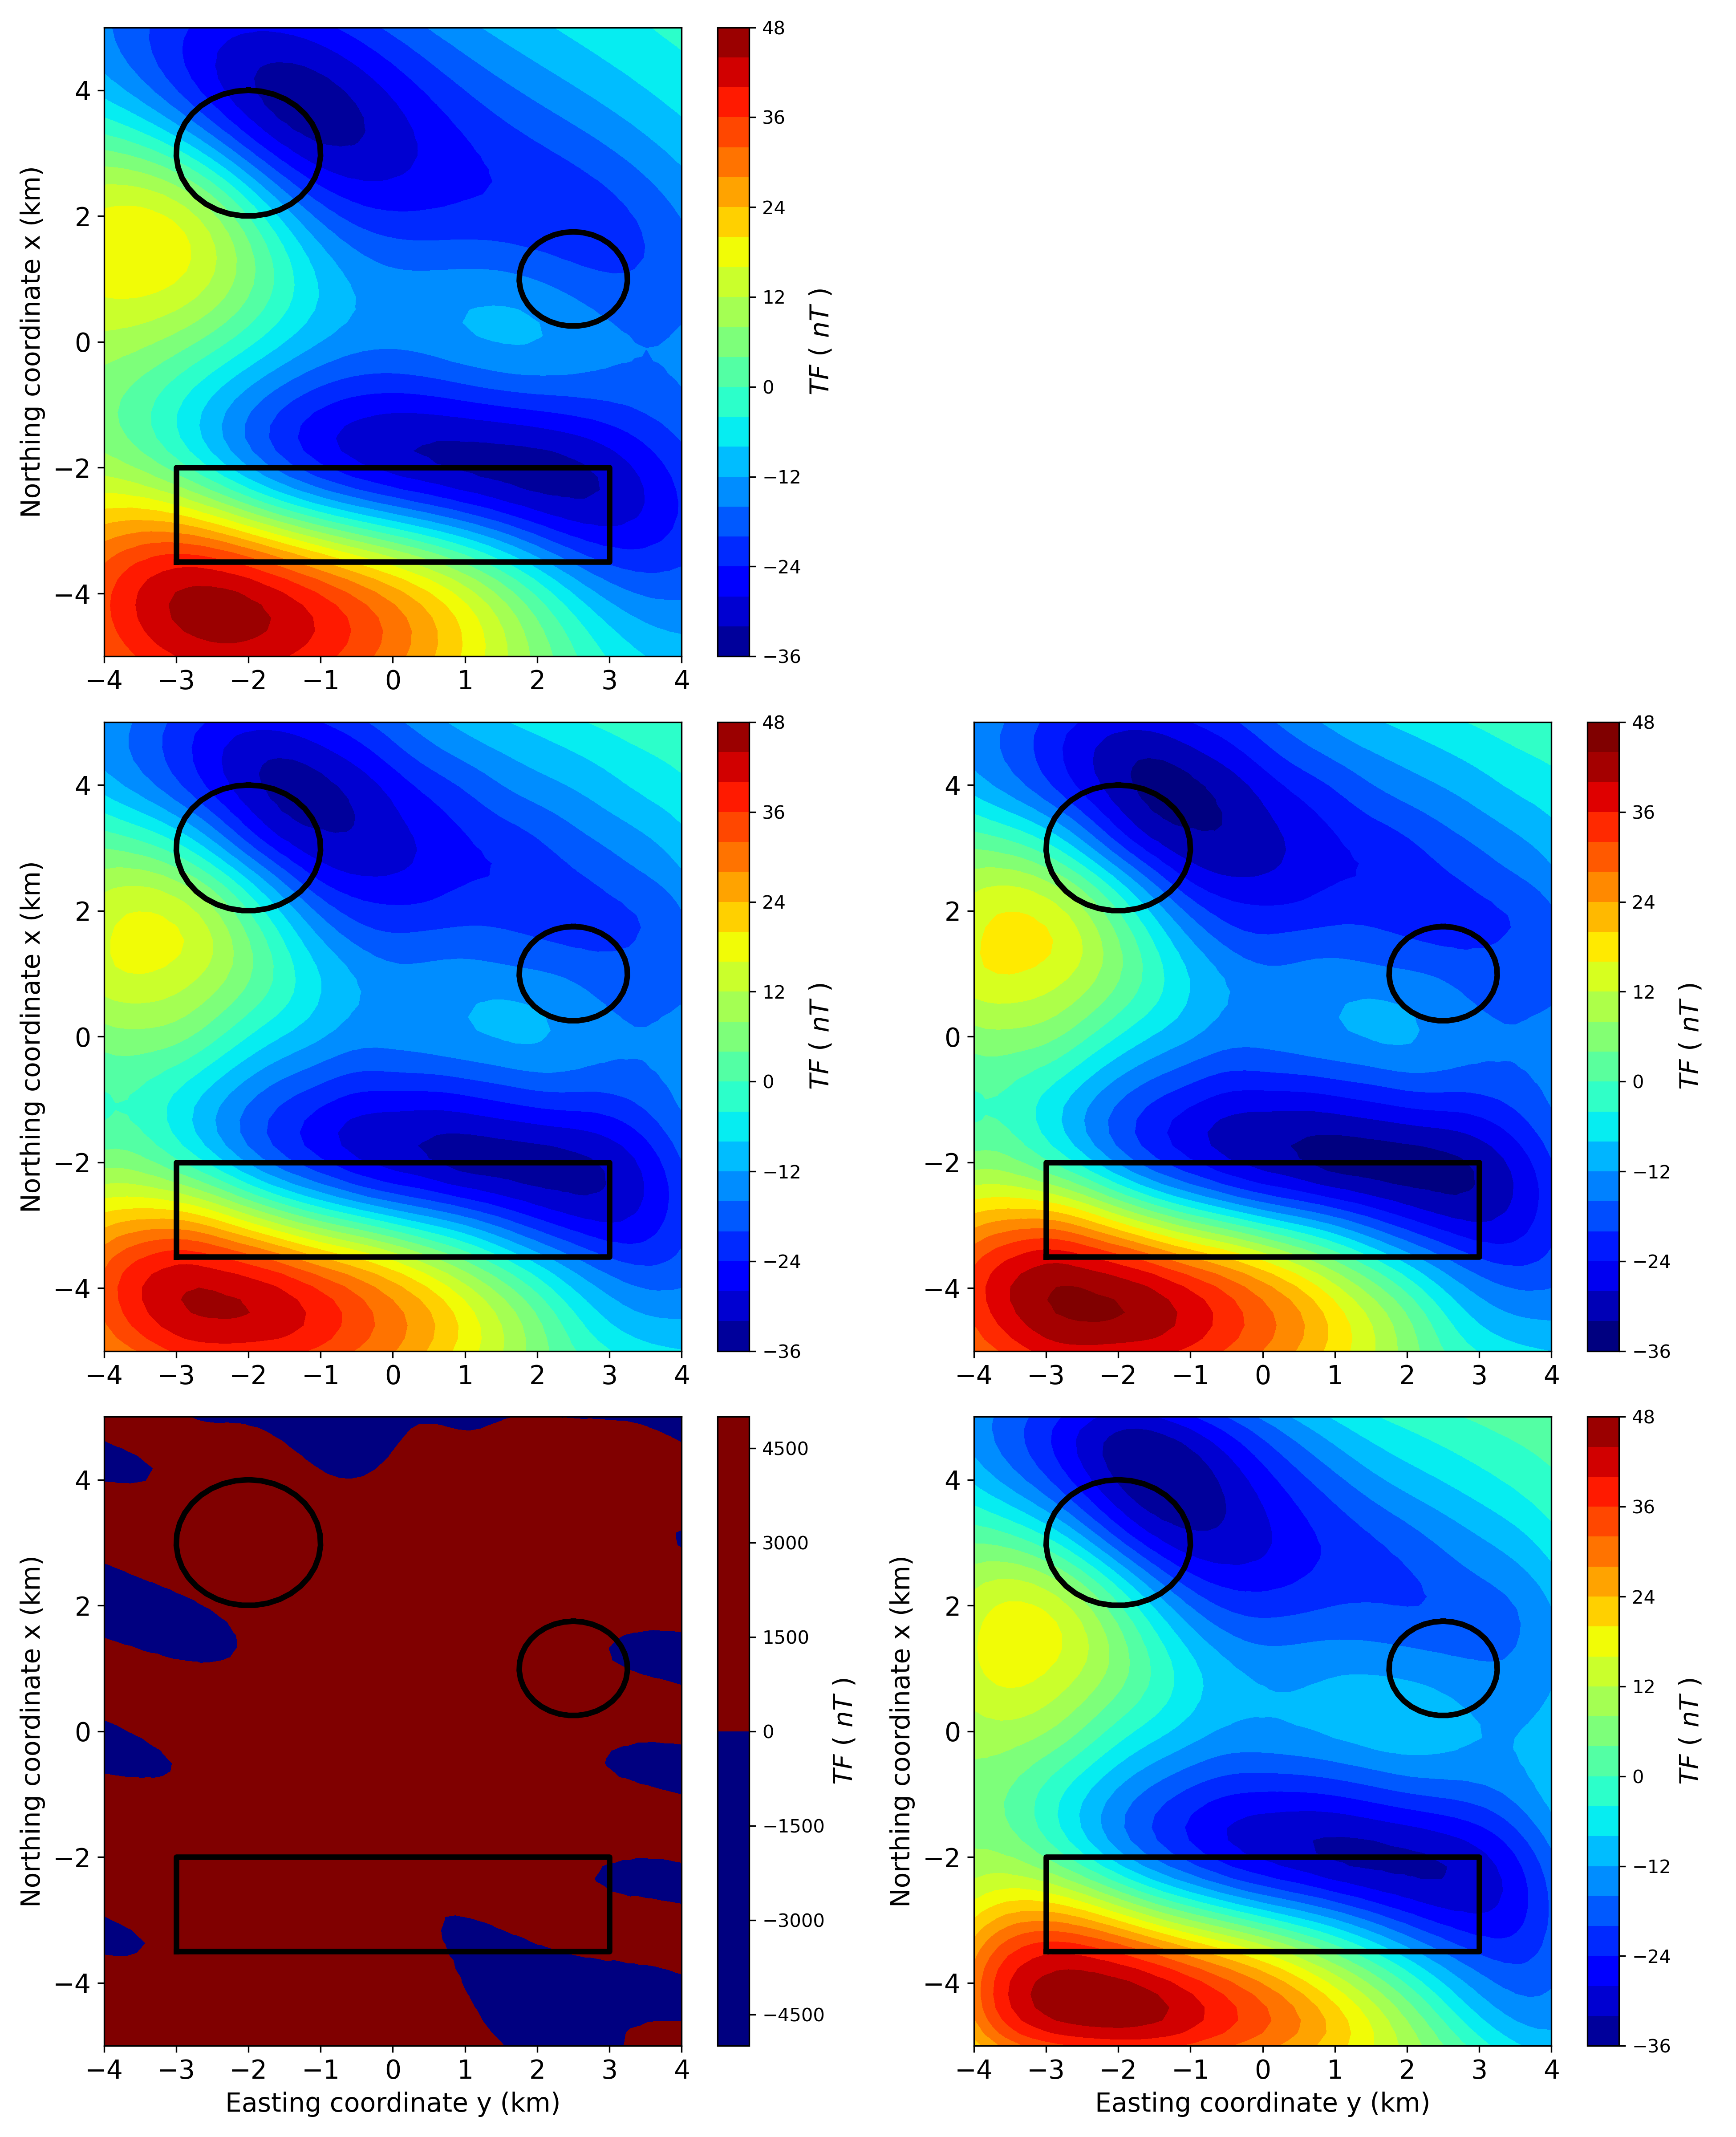
\includegraphics[width=10cm]{Fig/mag_upward}
	\end{center}
	\caption{True noiseless upward magnetic data at $z_i = -1400$ m height and predicted data for different methods of the equivalent layer with maximum level of noise. Panel \textbf{(A)} is the true upward magnetic data, Panel \textbf{(B)} is the classical method, \textbf{(C)} is the convolutional, \textbf{(D)} is the deconvolutional, \textbf{(E)} is the deconvolutional method using Wiener stabilization with a optimal value for $\mu = 10^{-13}$.}
	\label{fig:mag_up}
\end{figure}

\begin{figure}[htbp]
	\begin{center}
		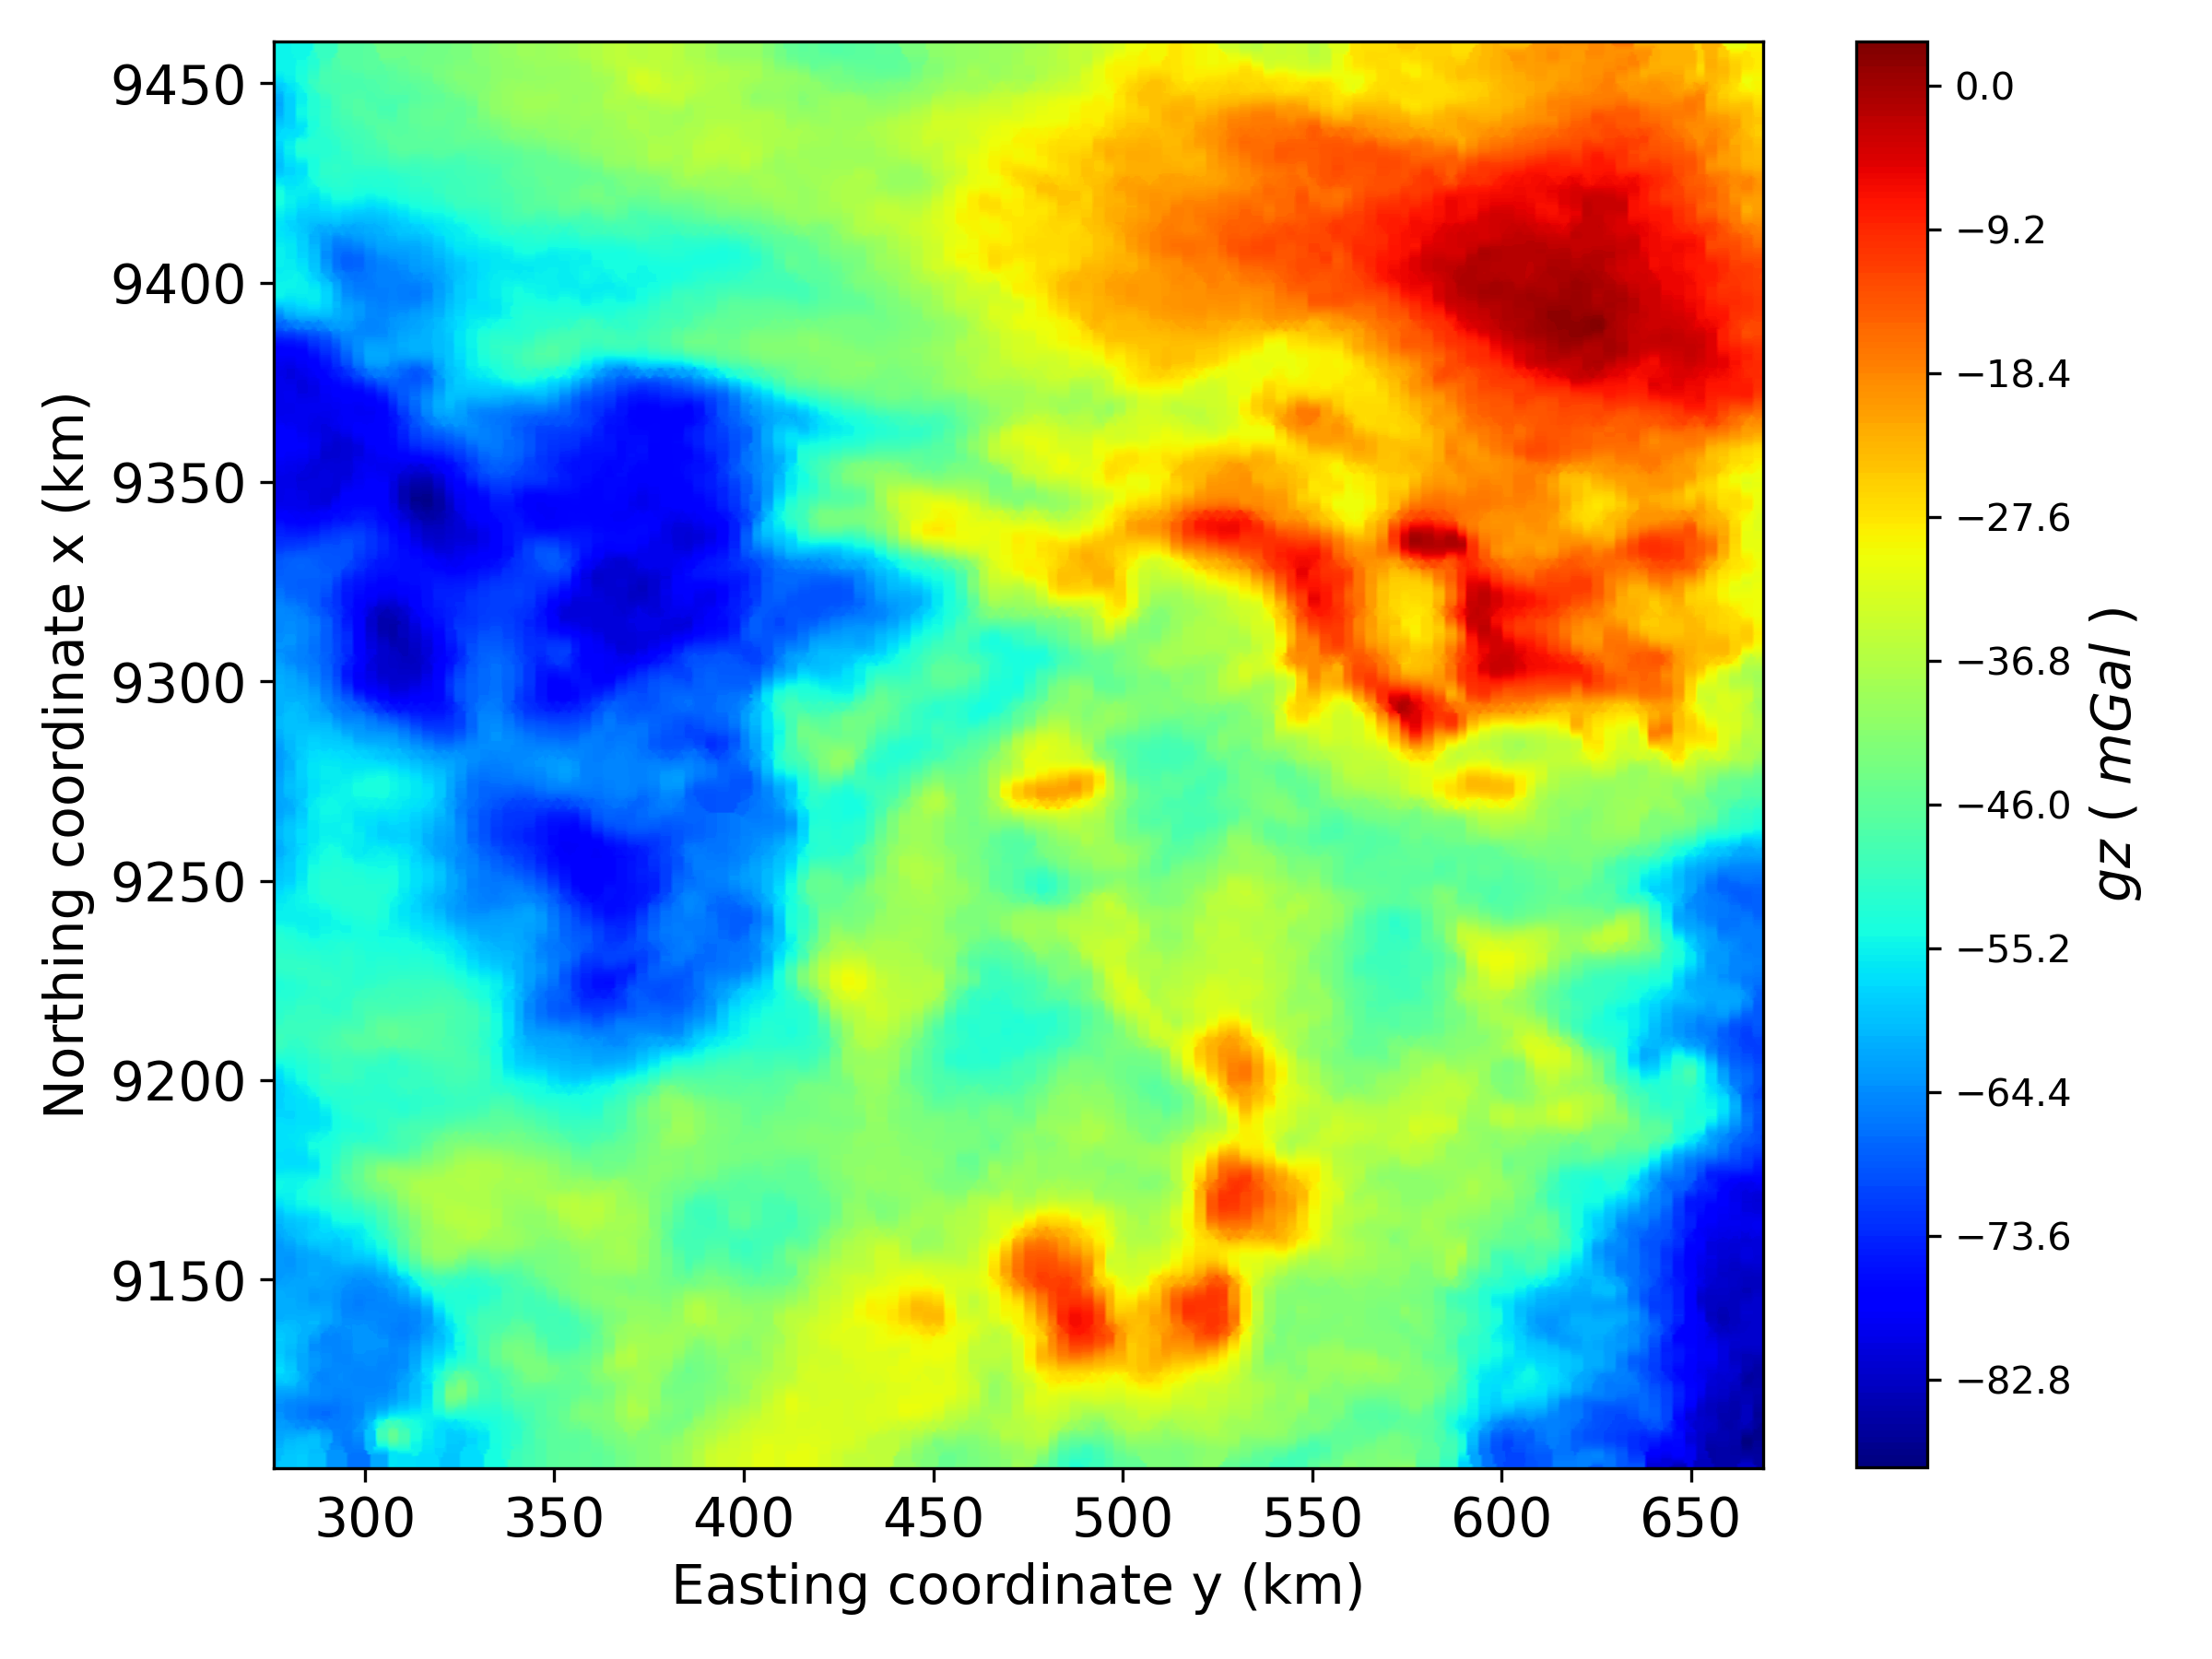
\includegraphics[width=10cm]{Fig/carajas_gz_real_data_1000x500}
	\end{center}
	\caption{Gridded real aerogravimetric data from Carajás, Brazil. A regular grid of $1,000 \times 500$ is being used, totalizing $N,M = 500, 000$ obsevation points and equivalent sources.}
	\label{fig:9}
\end{figure}

\begin{figure}[htbp]
	\begin{center}
		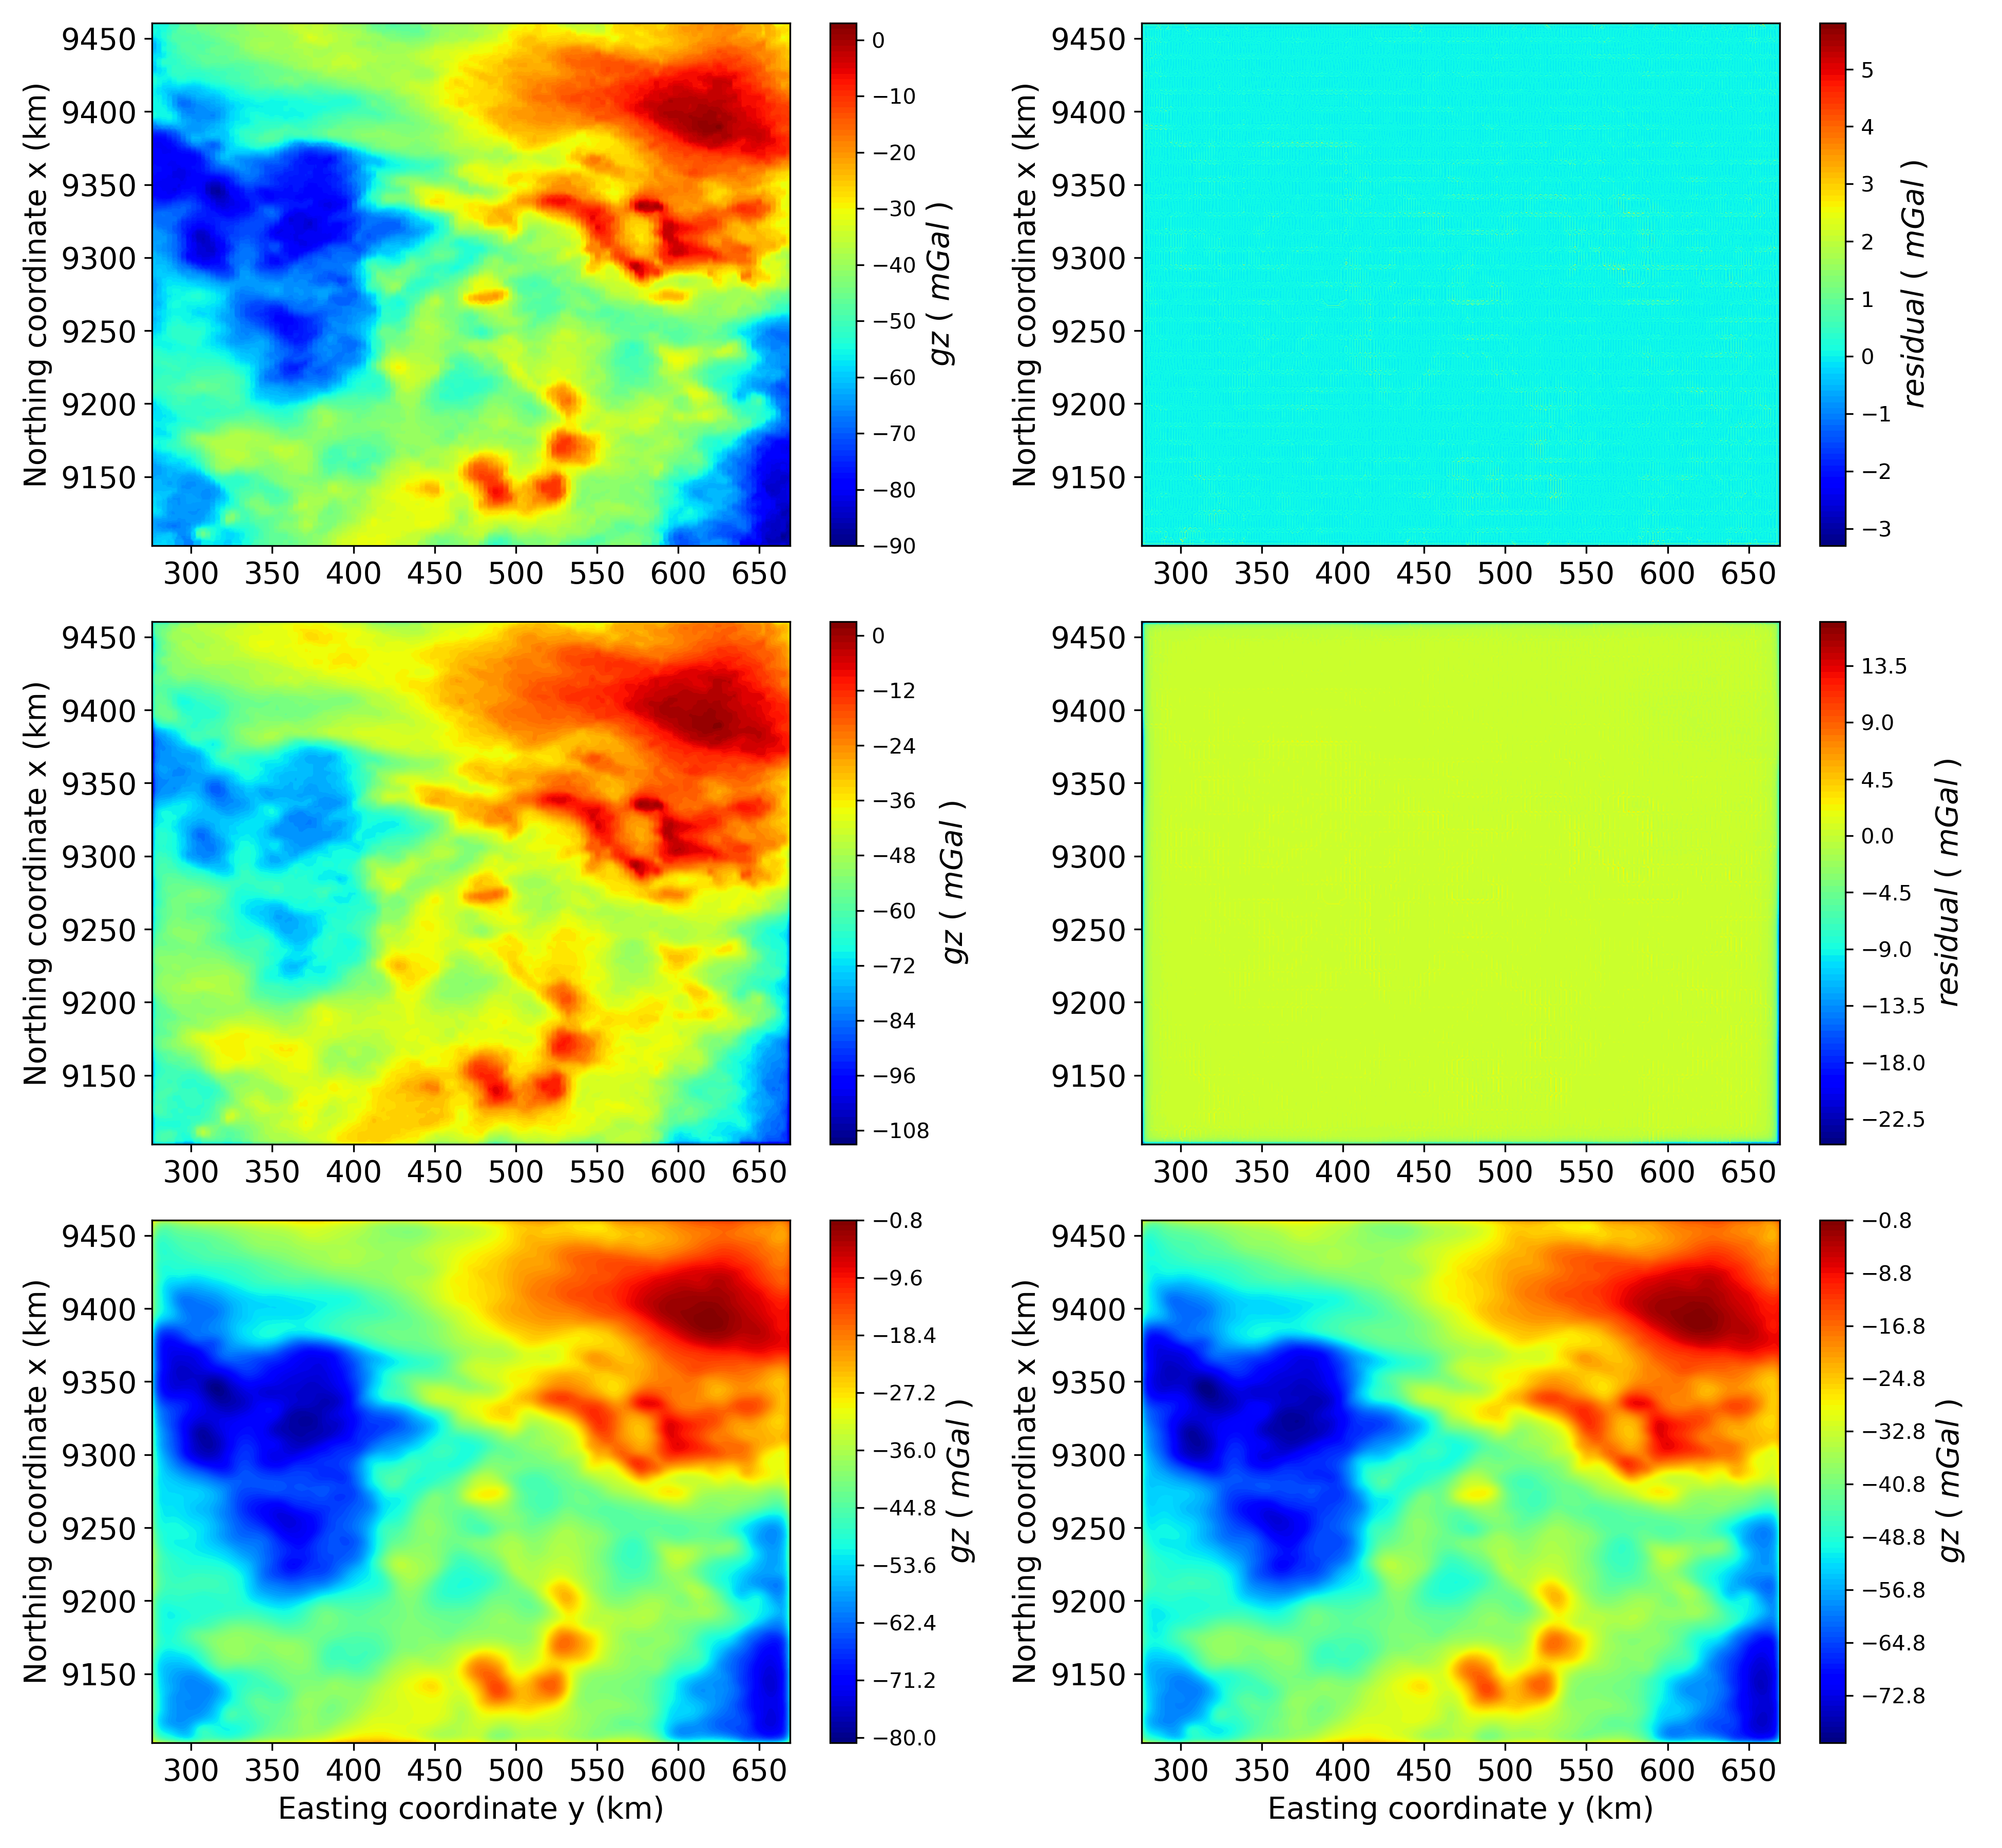
\includegraphics[width=10cm]{Fig/carajas_gz_predito_1000x500}
	\end{center}
	\caption{Panel \textbf{(A)} shows the Carajás predicted gravimetric data from convolutional equivalent layer method. Panel \textbf{(B)} shows the residual from the convolutional equivalent layer method. Panel \textbf{(C)} shows the predicted data from deconvolutional equivalent layer method. Panel \textbf{(D)} shows the residual from the deconvolutional equivalent layer method. Panel \textbf{(E)} shows the upward continuation at $z_i = -3500$ m for the convolutional method and Panel \textbf{(F)} shows the upward continuation at $z_i = -3500$ m for the deconvolutional method.}
	\label{fig:10}
\end{figure}

\begin{figure}[htbp]
	\begin{center}
		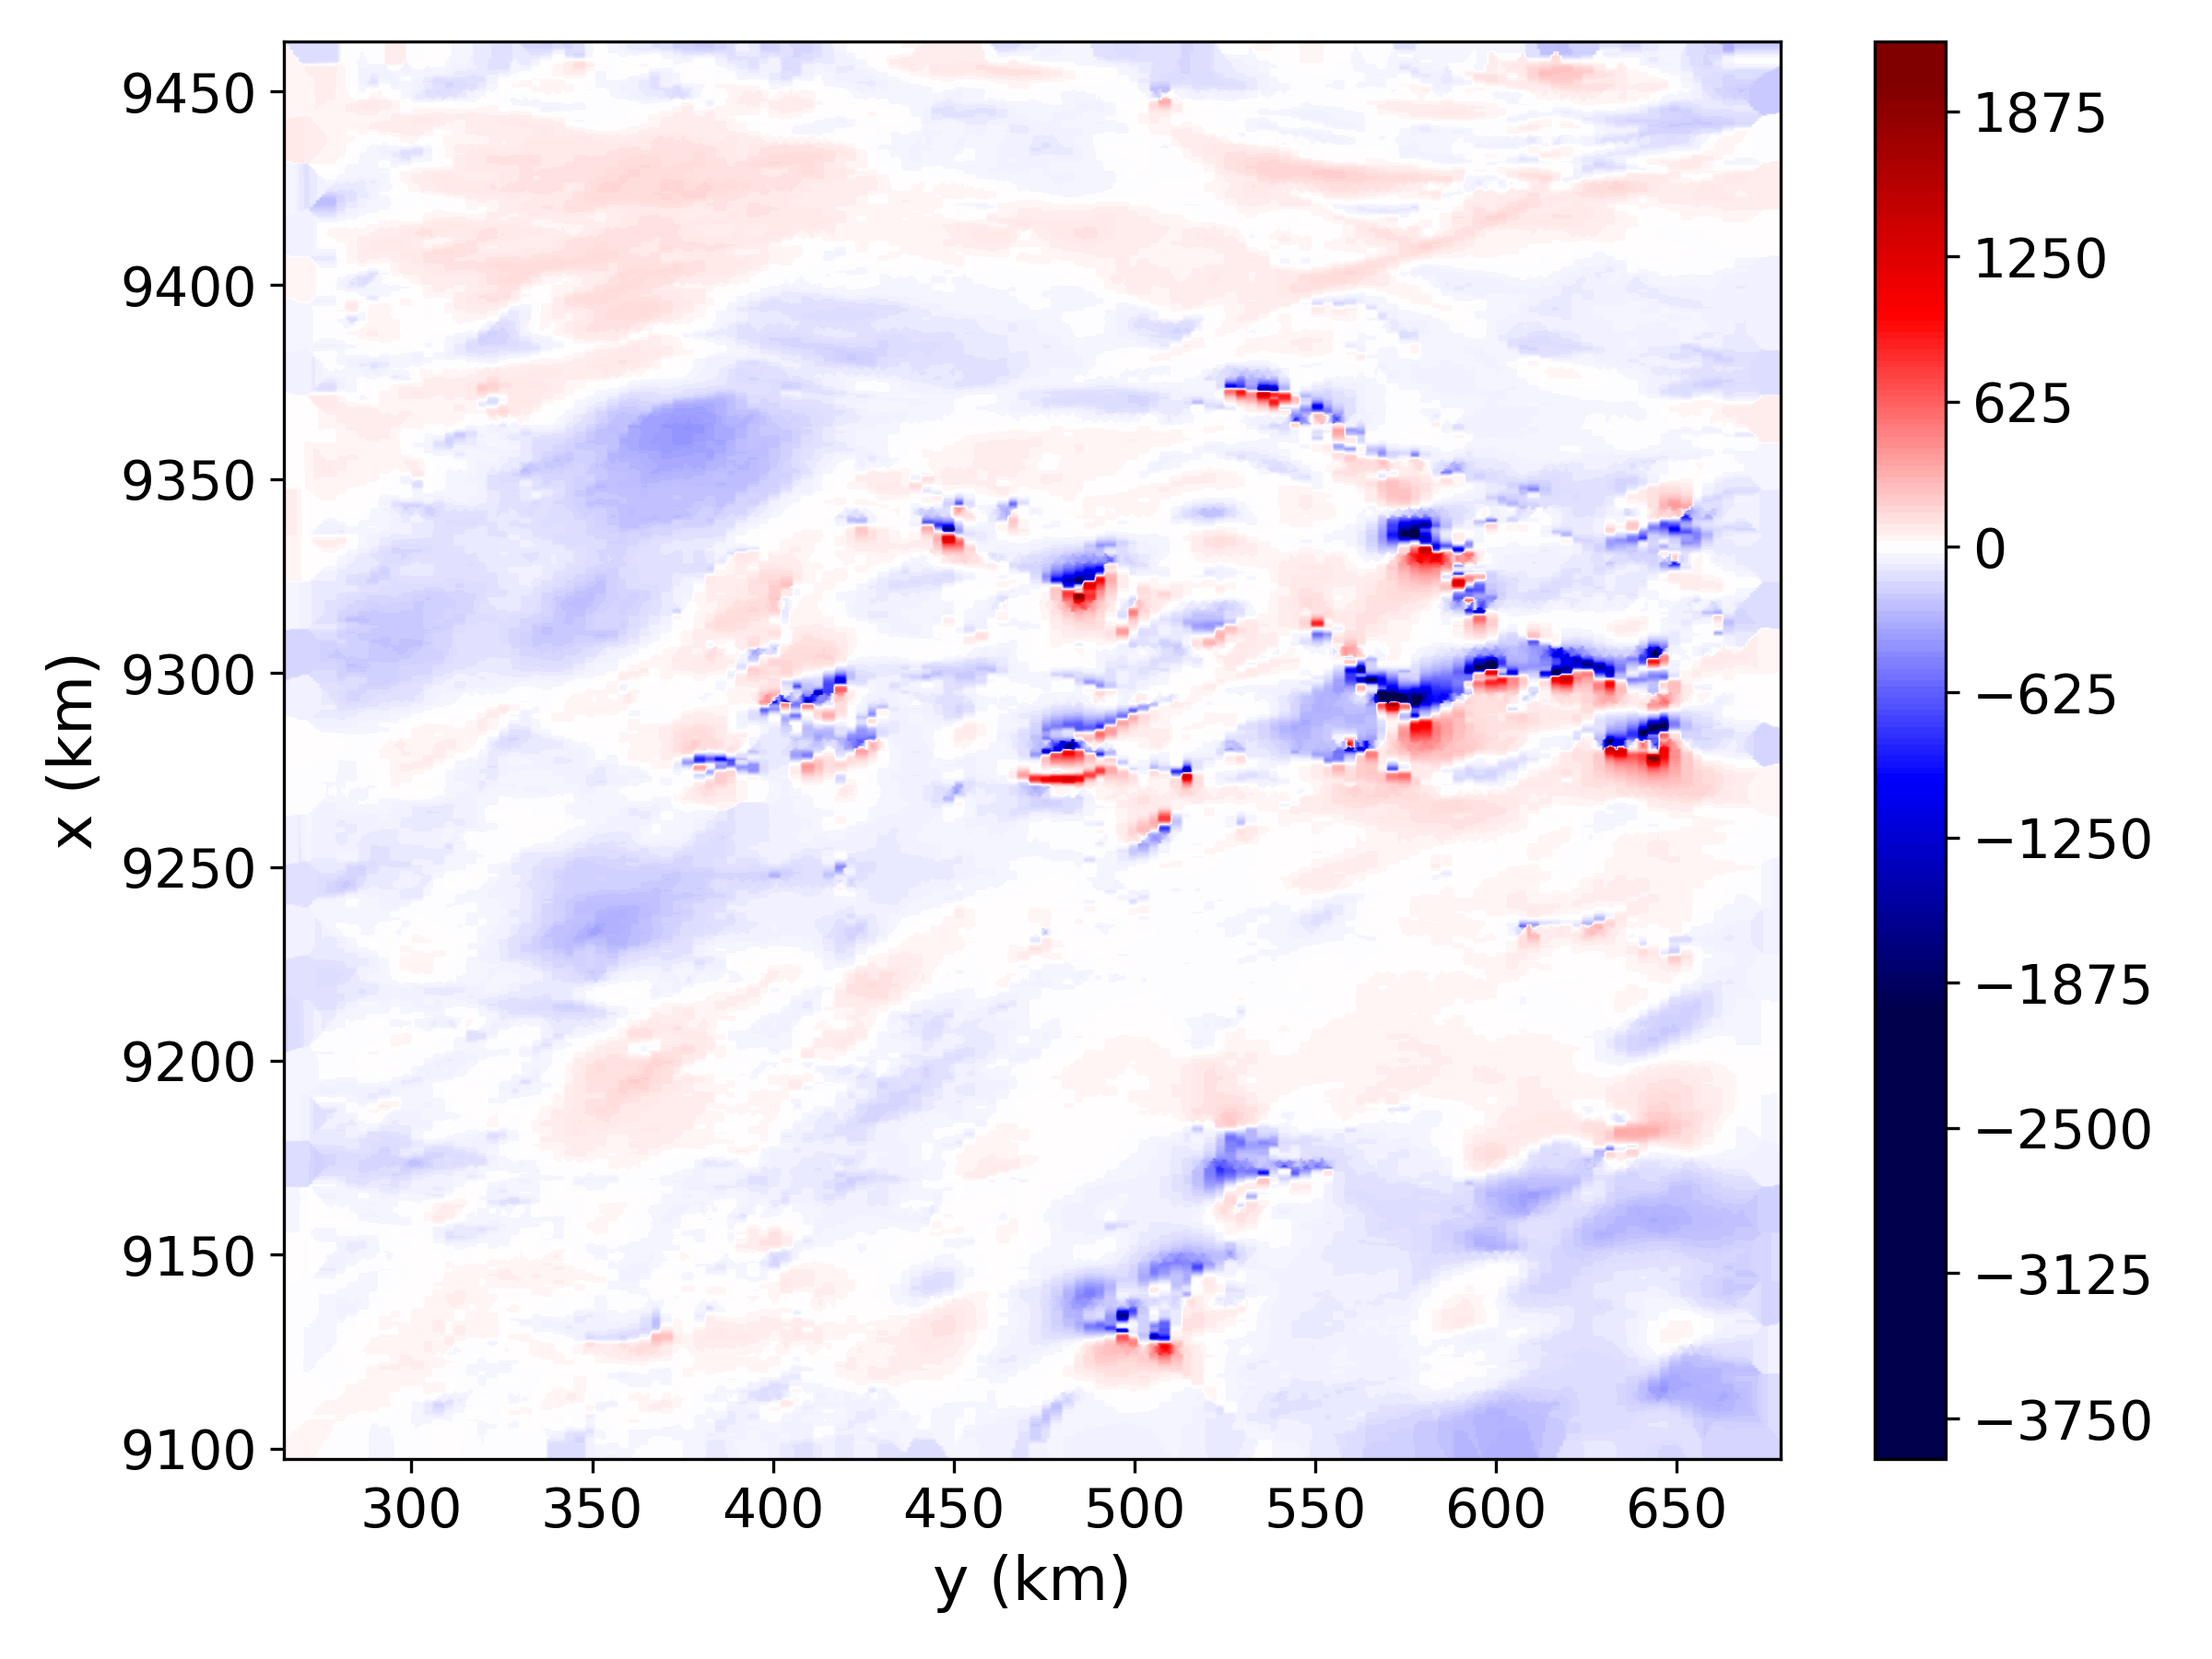
\includegraphics[width=10cm]{Fig/carajas_tf_real_data_1000x500}
	\end{center}
	\caption{Gridded real aeromagnetic data from Carajás, Brazil. A regular grid of $1,000 \times 500$ is being used, totalizing $N,M = 500, 000$ obsevation points and equivalent sources.}
	\label{fig:11}
\end{figure}

\begin{figure}[htbp]
	\begin{center}
		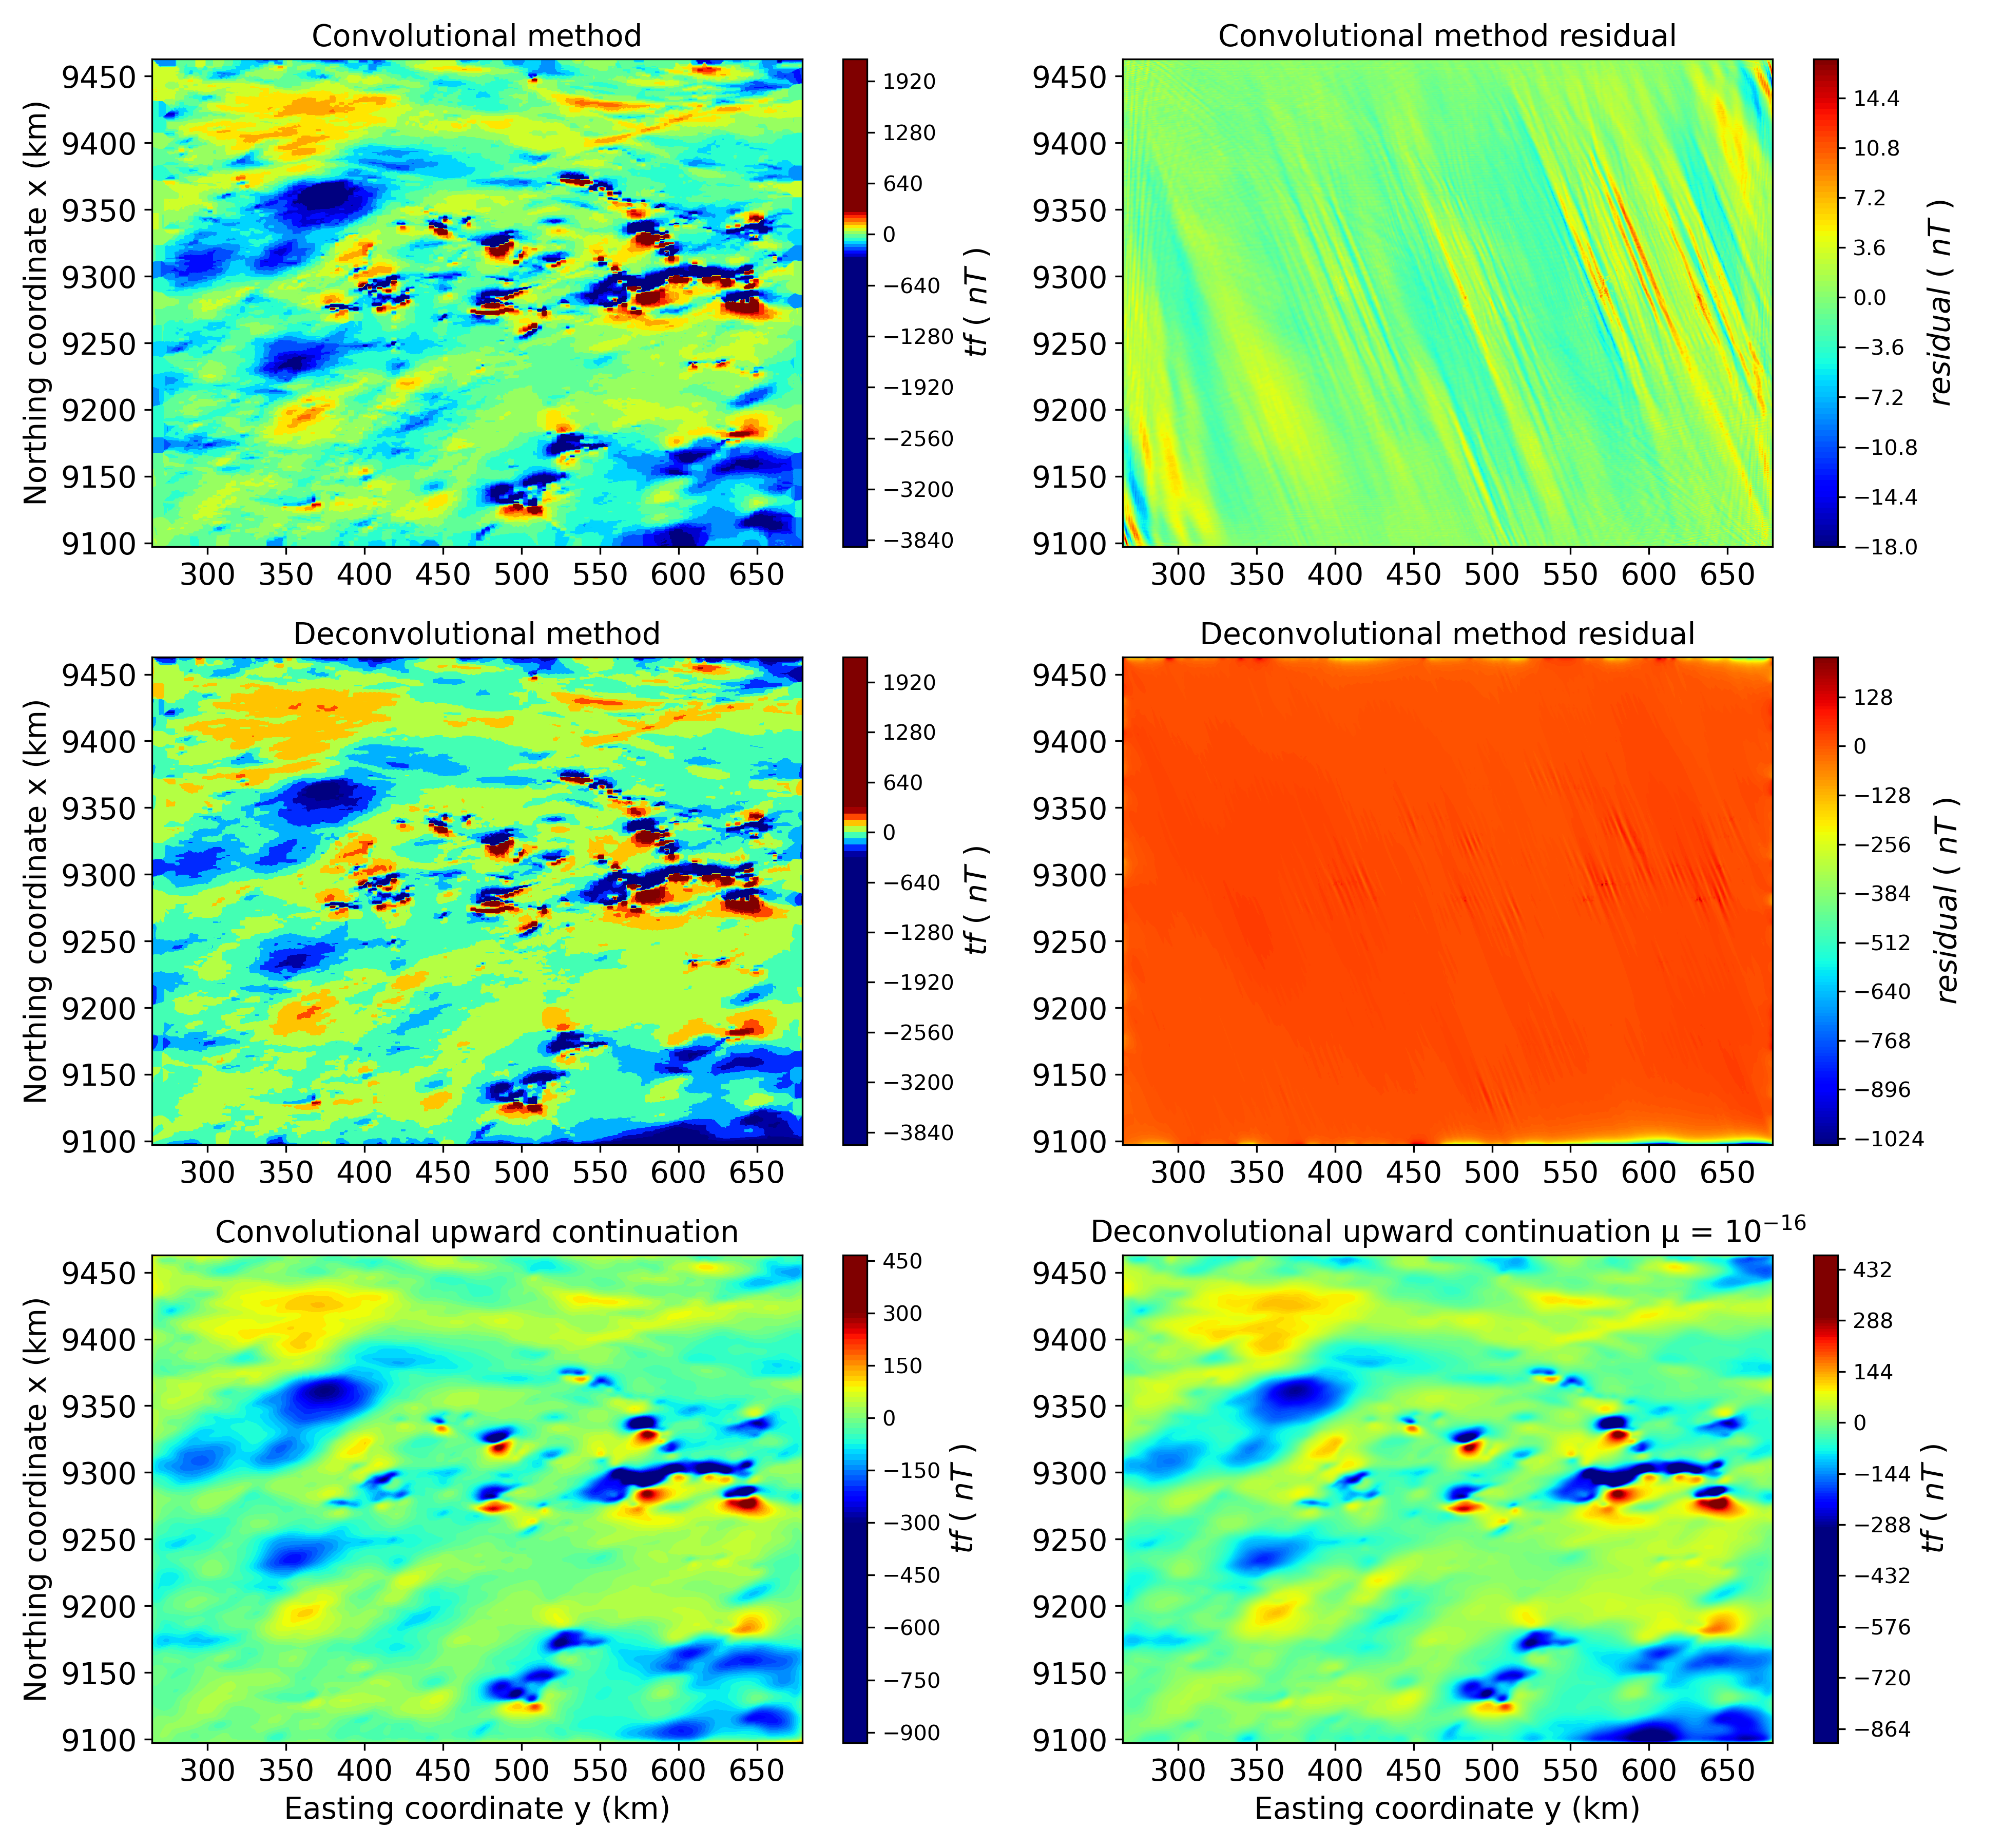
\includegraphics[width=10cm]{Fig/carajas_tf_predito_1000x500}
	\end{center}
	\caption{Panel \textbf{(A)} shows the Carajás predicted magnetic data from convolutional equivalent layer method. Panel \textbf{(B)} shows the residual from the convolutional equivalent layer method. Panel \textbf{(C)} shows the predicted data from deconvolutional equivalent layer method. Panel \textbf{(D)} shows the residual from the deconvolutional equivalent layer method. Panel \textbf{(E)} shows the upward continuation at $z_i = -3500$ m for the convolutional method and Panel \textbf{(F)} shows the upward continuation at $z_i = -3500$ m for the deconvolutional method.}
	\label{fig:12}
\end{figure}

%%% If you are submitting a figure with subfigures please combine these into one image file with part labels integrated.
%%% If you don't add the figures in the LaTeX files, please upload them when submitting the article.
%%% Frontiers will add the figures at the end of the provisional pdf automatically
%%% The use of LaTeX coding to draw Diagrams/Figures/Structures should be avoided. They should be external callouts including graphics.


%\bibliographystyle{frontiersinSCNS_ENG_HUMS} %  for Science, Engineering and Humanities and Social Sciences articles, for Humanities and Social Sciences articles please include page numbers in the in-text citations
%\bibliographystyle{frontiersinHLTH&FPHY} % for Health and Physics articles
%\bibliography{test}

%\end{document}
